\chapter{Optical Modelling and Design Analysis}
\label{Cap:Opt}

\section{Aims and objectives}

The aim of this chapter is to define the design of a concentrating collector for an air heating system using ray tracing optical analysis. The specific objectives are to:

\begin{itemize}[topsep=5pt,partopsep=0pt] \itemsep0pt
%\setlength\itemsep{0pt}
	\item Develop a ray tracing technique in 3D and implement the optical model in Matlab$^{\circledR}$;
	%\item Implement an optical model algorithm in Matlab$^{\circledR}$;
	\item Evaluate the effect of the parabolic reflectors and the tertiary cavity geometry on the optical performance;
	\item Assess the impact of the concentrator's length on reflector cost;
	\item Analyse the influence of the glazing inclination on the light transmittance through the glazed aperture;
	\item Characterise the optical profile of a concentrator used for experimental tests.
	%\item Specify the proposed concentrator's design to be used in this work;
	%\item To compare the energy distribution along the absorber between 2D and 3D ray tracing model;
	%\item To validate the 2D ray tracing model with a laser test.
\end{itemize}

\section{Design considerations of the concentrator}

\subsection{Overall assembly}

The proposed solar concentrator combines of an inverted absorber with an asymmetric compound parabolic concentrator (ACPC). It comprises: i) two parabolic reflectors; ii) a circular reflector; iii) two straight reflectors; iv) two end reflectors; v) a glazing cover not coincident to the aperture, and; vi) an transpired absorber plate. The entire collector is oriented south. A full drawing and cross-section are shown in Figures \ref{collector3D} and \ref{CSview}, respectively. 

\Figure[scale=0.40,placement=!ht,label={collector3D},caption={Concentrator's design in 3D.}]{figs/collector3D.PNG}

\Figure[scale=0.70,placement=!ht,label={CSview},caption={Concentrator's cross section view.}]{figs/CSview2.eps}

\subsection{Glazing position}
The glazing placed from the aperture confines heated air in the collectors, as well as offering protection for the collector interior against weather conditions (\cite{Shams2016}). Its position at a given inclination $\beta$ (shown in Figure \ref{CSview}) seeks to gain solar energy transmittance and reduce light reflection.

\subsection{Aperture position}
The concentrator's aperture is set at the vertical position (at the truncation line in Figure \ref{CSview}) so that shading can be avoided when two or more collectors are stacked on a vertical wall enabling the full fa\c{c}ade area available to be harnessed.

\subsection{Parabolic shape}
The angles of both parabolas axes ($\theta_{\!_{\rm{P1}}}$ and $\theta_{\!_{\rm{P2}}}$) shown in Figure \ref{CSview} define the parabolic shape, therefore affecting size, angular acceptance range (\cite{Zacharopoulos2000}; \cite{Harmim2012}) and maximum geometric concentration ratio (\cite{Mills1978}). Given the same level of concentration ratio, concentrators of narrow angular acceptance are more efficient so collect higher amounts of the available solar energy (\cite{Sarmah2011}).
    
%\subsection{Truncation level}
%Truncation is an effective way to reduce reflector costs and collector's size but receiving less solar radiation. The effect of this on concentration ratio, height-aperture width ratio and reflector length has been studied extensively (\cite{Rabl1976}; \cite{McIntire1979}). Truncated concentrators accept solar rays at broader incident angles due to reduction of reflections, then more of the available solar energy is collected (\cite{Carvalho1985}).
    
%\subsection{Length and end effect}
%If a linear concentrator is long in an east-west orientation compared to its width and height, it can be assumed to behave as a two dimensional system where end effects are negligible (\cite{Eames1993a}). For concentrators with short axial lengths, the end losses need to be included on the optical analysis as a portion of reflected solar rays may not reach the absorber under certain obtuse solar incident angles. End loss factors dependent on the incident angle have been analytically calculated for imaging parabolic troughs (\cite{Rabl1985}) and for linear Fresnel concentrators (\cite{Pu2011}; \cite{Heimsath2014}; \cite{Hongn2015}).
    
\subsection{Cavity height}
The cavity contributes to the formation of thermally stratified air layers below the absorber that suppresses convective and radiative heat losses. The height of this cavity affects the distribution of incoming solar radiation along the absorber surface in a way to enhance heat transfer mechanism and mitigate hot spots.

\section{Operation conditions}

This solar air heating system is designed to operate in Dublin, Ireland, where the latitude ($\phi$) is 53.35$^{\circ}$ and the longitude is -6.26$^{\circ}$ over the summer season (from 21/06 to 21/09) for 8 hours per day, from 9 am to 5 pm (local time).

Defining the operating constraint is an essential prerequisite to calculate the sun angles applicable to the period of operation. They are obtained using solar time ($\rm{t_{st}}$), which does not coincide with the local standard time. The relationship between solar and local times, given by Eq. (\ref{solartime}), is due to the deviation between the local longitude and the chosen meridian on which the local standard time is based.

\begin{equation}
    \mathrm{t_{st} = t_{\!_{LST}} + \frac{4(\ell_{st} - \ell_{local}) + E_T}{60}}
    \label{solartime}
\end{equation}

Irregularity of the earth's motion around the sun, accounted by the "Equation of Time" ($\rm{E_T}$) as a function of the year's day (\cite{Goswami2015}). Solar hour angles ($\omega_{\rm{s}}$) were obtained from the solar time for each day of operation. 

%The solar altitude and solar azimuth angles (${\rm a_s}$ and $\gamma_{\rm{s}}$) were calculated from (\cite{Duffie2013}):
%
%\begin{equation}
%\mathrm{{a_s} = {\sin ^{ - 1}}\left( {\sin \phi \sin {\delta _s} + \cos \phi \cos {\delta _s}\cos {\omega_s}} \right)}
%\label{solar_alt}
%\end{equation}
%\vspace*{-0.5cm}
%\begin{equation}
%\mathrm{\gamma_s = {\sin^{-1}}\left(\frac{\cos \omega_s \sin \delta_s}{\cos a_s}\right)}
%\label{azimuth}
%\end{equation}
%
%\noindent where the solar declination $\delta_{\rm{s}}$ is a function of the year's day.

A solar position plot of ${\rm a_s}$ against $\gamma_{\rm{s}}$ at the latitude of Dublin is shown in Figure \ref{Alt_Azz}, where each graph corresponds to a particular day in the operation period. The values of ${\rm a_s}$ and $\gamma_{\rm{s}}$ at any point in time in the operation period were used as inputs in the optical modelling. The calculation of these solar angles was verified by Sun calculators available on the Internet (\cite{Time2018}; \cite{SunCalc2018}).

\Figure[scale=0.60,placement=!ht,label={Alt_Azz},caption={Solar position diagram for 53.35$^{\circ}$ of latitude.}]{figs/Alt_Azz2.eps}

Over the period of operation, the calculated limits of altitude solar angle were 60.1$^{\circ}$ when the Sun is at its highest altitude, on 21/06 at noon; and 14.6$^{\circ}$ when the Sun is at its lowest altitude in the last day of summer (21/09) at 9am. The collector must therefore accept direct solar radiation within the solar altitude range, from 15$^{\circ}$ to 61$^{\circ}$.

\section{Reflector's design specification}

%\subsection{Software tools used}

%This section describes how the reflectors were designed and placed to form the proposed air heating concentrator. The design was performed in Matlab$^{\circledR}$ with the help of SolidWorks$^{\circledR}$ by using positive x-y coordinates.

\subsection{Parabolic reflectors design}

To design the parabolic reflectors, the first step was to define the equation of the parabola whose axis is coincident to the y-axis with the vertex set at the origin:

\begin{equation}
\mathrm{{y_p} = \left( {\frac{1}{{4f}}} \right){x_p}^2}
\label{parabola}
\end{equation}

\noindent where f is the focal distance, given by Eq. (\ref{focal}) (\cite{Winston2005}):

\begin{equation}
\mathrm{f = \frac{{{W_{abs}}}}{2}\left( {1 - \cos {\theta_{a}}} \right)}
\label{focal}
\end{equation}

\noindent and $\rm{\theta_{a}}$ is angle related to position of the parabola. The next step was to translate and rotate the parabola to form the parabolic section. Both parabolas were designed and placed at the correct position using basic tools from SolidWorks$^{\circledR}$ as shown in Figure \ref{rottrans_two}. The expressions for calculating $\rm{\theta_{a}}$, $\rm{\Delta x}$ and $\rm{\Delta y}$ for each parabola are shown in Table \ref{parabolas}.

\begin{figure}[ht!]
	\begin{minipage}{0.49\columnwidth}
		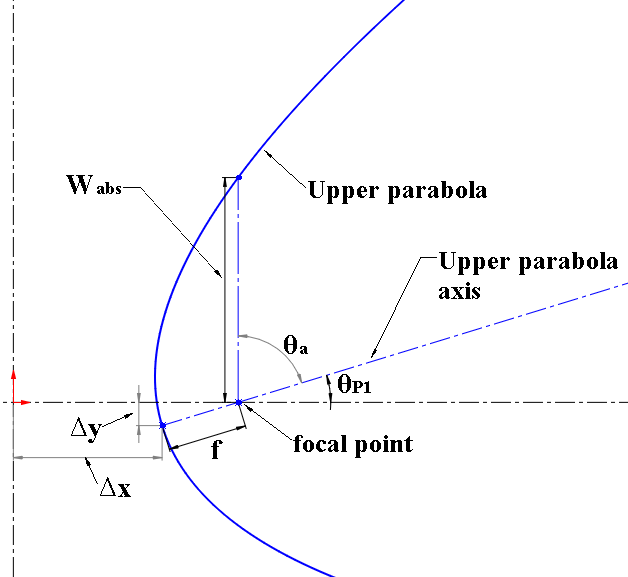
\includegraphics[width=0.9\columnwidth,height=6.0cm]{figs/upper_parabola.PNG}
		\subcaption{Upper parabola.}
	\end{minipage}
	\begin{minipage}{0.49\columnwidth}
		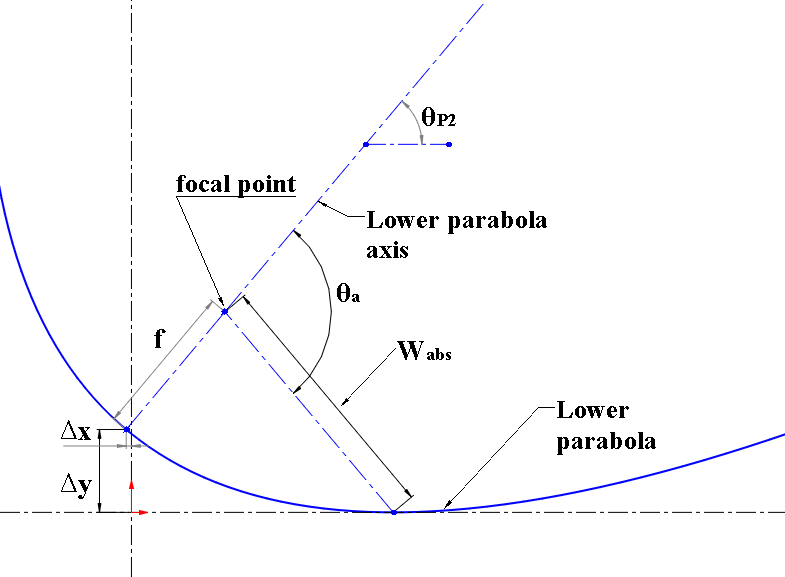
\includegraphics[width=0.9\columnwidth,height=6.0cm]{figs/lower_parabola.PNG}
		\subcaption{Lower parabola.}
	\end{minipage}
	\caption{(a) Upper and (b) lower parabolas placed at the final position.}
	\label{rottrans_two}
\end{figure}

\begin{table}[!ht]
	\centering
	\caption{Expressions for the parabolas' parameters.}
	\begin{tabular}{cp{3.3cm}l}
		\hline \\[-12pt]
		\vspace*{0.1cm} Parameter & Upper Parabola & Lower Parabola \\ [0pt]
		\hline \\[-12pt]
		$\theta_{{\rm{a}}}$ & $90 -\theta_{\!_{\rm{P1}}}$ & 2$\theta_{\!_{\rm{P2}}}$ \\ [5pt]
		%$\theta_{\!_{\rm{R}}}$ & 90 $- \alpha_{\!_{\rm{P1}}}$ & 90 $- \alpha_{\!_{\rm{P2}}}$ \\ [5pt]
		$\Delta \rm{x}$ & $\rm{{W_{abs}} - f\cos {\theta_{\!_{P1}}}}$ & $\rm{{W_{abs}} - ({W_{abs}} + f)\cos {\theta_{\!_{P2}}}}$ \\ [5pt]
		$\Delta \rm{y}$ & $\rm{- f\sin {\theta_{\!_{P1}}}}$ & $\rm{({W_{abs}} - f)\sin {\theta_{\!_{P2}}}}$ \\ 
		\hline 
	\end{tabular}
	\label{parabolas}
\end{table}

The next step was to arrange the parabolas properly in a common coordinate system to form the full untruncated parabolic section shape APQD, shown in Figure \ref{twoparabolas22}. In this case, point D intercepts the x-axis and the vertical segment length AD is equal the absorber width ($\rm{W_{abs}}$), as it is the section end. The full aperture indicated by the segment PQ is obtained according to the parabola axes angles. The aperture was set to be vertical, therefore the section is truncated at the line indicated by the segment BC. The curves AB and DC then represent the shapes of the upper and lower reflectors, respectively. Their coordinate limits are given in Table \ref{coordinates}.

\Figure[scale=0.55,placement=!ht,label={twoparabolas22},caption={Two parabolas arranged to form the truncated parabolic section (ABCD). Dashed curves of the parabolas were eliminated.},shortcaption={Two parabolas assembled to form the truncated parabolic section (ABCD)}]{figs/fig_primary3.PNG}

\begin{table}[!ht]
	\centering
	\caption{Reflector coordinate limits.}
	\begin{tabular}{lll}
		\hline \\[-12pt]
		\vspace*{0.1cm} Reflector & x limits & y limits \\ [0pt]
		\hline \\[-12pt]
		Upper & $\rm{{W_{abs}} \le {x} \le {x_{apt}}}$ & $\rm{{W_{abs}} \le {y} \le {y_{apt,upper}}}$ \\ [5pt]
		Lower & $\rm{{W_{abs}} \le {x} \le {x_{apt}}}$ & $\rm{0 \le {y} \le {y_{apt,lower}}}$ \\ 
		\hline 
	\end{tabular}
	\label{coordinates}
\end{table}

%The mathematical process of rotation and translation was achieved using the Affine transformation technique (\cite{Duffy2016}), which consists of applying a matrix multiplication as shown in Eq. (\ref{affine}):
%
%\begin{equation}
%\left[ {\begin{array}{*{20}{c}}
%		\mathrm{{{x }}}\\
%		\mathrm{{{y }}}\\
%		1
%		\end{array}} \right] = \left[ {\begin{array}{*{20}{c}}
%		1&0&\mathrm{\Delta x}\\
%		0&1&\mathrm{\Delta y}\\
%		0&0&1
%		\end{array}} \right]\left[ {\begin{array}{*{20}{c}}
%		\mathrm{\cos {\theta_{\!_R}}}&\mathrm{\sin {\theta_{\!_R}}}&0\\
%		\mathrm{- \sin {\theta_{\!_R}}}&\mathrm{\cos {\theta_{\!_R}}}&0\\
%		0&0&1
%		\end{array}} \right]\left[ {\begin{array}{*{20}{c}}
%		\mathrm{{{ x_p }}}\\
%		\mathrm{{{ y_p }}}\\
%		1
%		\end{array}} \right]
%\label{affine}
%\end{equation}
%
%\noindent with the parameters $\rm{\Delta x}$ and $\rm{\Delta y}$ as the displacements in x and y, respectively, $\rm{\theta_{\!_R}}$ as the angle of rotation (which is the complement of the parabola axis angle), and $\rm{{{x}}}$ and $\rm{{{y}}}$ are the new coordinates of the parabola calculated by the Affine transformation technique. 
%
%The mathematical equation to represent a rotated-translated parabola is implicit defined by an irreducible polynomial of second degree, which is complex solve for ray tracing applications. Another way of representing the portion of the parabolic reflectors was thus used to approximate the parabolic shapes to a $\rm{N_d}^{\rm{th}}$ degree polynomial fit  in the form of:
%
%\begin{equation}
%\mathrm{y = \sum\limits_{j = 0}^{N_d} {{a_j}x^j}}
%\label{eqP1}
%\end{equation}
%
%\noindent where the linear coefficients $\rm{a_{\!_{0}}}$, $\rm{a_{\!_{1}}}$, $\rm{a_{\!_{2}}}$, $\rm{a_{\!_{3}}}$, ..., $\rm{a_{\!_{Nd}}}$ and the degree order $\rm{N_d}$ were determined in a way to maximise the fit using a linear least-squares solver with linear constraints.

The equations used to model the parabolas consider x and y as function of a new parametric variable $\rm{t_p}$ assigned for each parabolic shape, as shown in Eqs. (\ref{p_x}) and (\ref{p_y}). These parametric equations model the exact parabolic shapes and are quadratic polynomials in $\rm{t_p}$, which takes minimum process time to be solved. 

\begin{equation}
	\mathrm{x = \frac{1}{4f}\sin\theta_a t_{p}^2 + \cos\theta_a t_p + \Delta x}
	\label{p_x}
\end{equation}
\vspace*{-0.75cm}
\begin{equation}
	\mathrm{y = \frac{1}{4f}\cos\theta_a t_{p}^2 - \sin\theta_a t_p + \Delta y}
	\label{p_y}
\end{equation}

\noindent where the parametric variables range to provide x and y coordinates whose limits are established in Table \ref{coordinates}.

\subsection{Circular reflector design}

For this circular reflector, a quarter of a circle was used, whose centre was set at \mbox{($\rm{W_{abs}}$, $\rm{W_{abs}}$)} and radius $\rm{W_{abs}}$. Eq. (\ref{quartercircle}) expresses the calculation for the circular section obtained:

\begin{equation}
	\mathrm{{y} = {W_{abs}} - \sqrt {\mathrm{W_{abs}^2 - {{\left( {{x} - {W_{abs}}} \right)}^2}}}}
	\label{quartercircle}
\end{equation}

\noindent where the coordinate limits are $\rm{0 \le {x} \le {W_{abs}}}$ and $\rm{0 \le {y} \le {W_{abs}}}$. The shape of the circular sector is illustrated in Figure \ref{three_sections} by the curve DE. 

\subsection{Straight reflector design}

The straight reflector section comprises two vertically straight reflector of height $\rm{H_{\!_{TS}}}$ above the circular section and ends at the absorber surface (whose y-coordinate is $\rm{y_{\!_{TS}}}$). The coordinate limits here are $\rm{0 \le {x} \le {W_{abs}}}$ and $\rm{W_{abs} \le {y} \le {y_{\!_{TS}}}}$. In Figure \ref{three_sections} they are represented by the vertical segments EF and AG.
%, as shown in Figure \ref{TS_SS}.

\subsection{End reflectors design}

The end reflectors are two identical flat surfaces, one at each end of the concentrator (west and east sides shown in Figure \ref{collector3D}), where their boundaries are the shapes of the other reflectors altogether.

\subsection{Summary of overall coordinates}

Figure \ref{three_sections} illustrates all the reflectors arranged along with the main coordinates.

\Figure[scale=0.40,placement=!ht,label={three_sections},caption={Concentrator's cross section view with the appropriate coordinate information.}]{figs/three_sections.PNG}

Figure \ref{three_sections3D} shows the concentrator in three dimensions, where:

\begin{itemize}[topsep=5pt,partopsep=0pt] \itemsep0pt
\item AHIB and DKJC are the upper and lower parabolic reflectors;
\item ELKD is the circular reflector;
%\item ELMF and AHNG are the straight reflectors;
\item ABCDEFG and HIJKLMN are the western and eastern end reflectors, respectively;
\item FMNG is the absorber surface and BIJC is the aperture;
\item The concentrator’s main dimensions are: depth $\rm{W_{col}}$, height $\rm{H_{col}}$ and length $\rm{L_{col}}$.
\end{itemize}

\Figure[scale=0.60,placement=!ht,label={three_sections3D},caption={Final concentrator concept.}]{figs/collector3D-3.PNG}

\section{Ray Tracing and Optical Modelling}

Ray tracing techniques are algorithms to simulate sunlight rays passing through an optical system. Ray tracing analysis gives the optical performance for complex reflecting geometries considering both direct and diffuse solar radiation (\cite{Ali2013}). When a ray is incident on a reflecting surface, most of its energy will be reflected. In ray tracing, the law of reflection is applied in vector form (\cite{Winston2005}). As the IACPC is a complex geometry, there is no set of analytic equations for predicting its optical performance. A ray tracing technique is therefore employed to simulate the passage of direct radiation rays through the concentrator (\cite{Ali2013}). This analysis provides:

\begin{itemize}[topsep=5pt,partopsep=0pt] \itemsep0pt
	\item The average number of reflections before the incoming rays reach the absorber (\cite{Shams2013}; \cite{Benrejeb2016});
	\item The optical efficiency as a function of the incidence angle (\cite{Kothdiwala1996}; \cite{Souliotis2011});
	\item Visualisation of rays' path and reflection points (\cite{Mallick2007}; \cite{Ratismith2014}; \cite{Ustaoglu2016});
	\item The intensity of the incident energy distribution at the absorber (\cite{Sellami2013}; \cite{Ali2014}; \cite{Bellos2016});
	\item The system's optical characteristics as boundary conditions for detailed computational fluid dynamics (\cite{Mallick2007}; \cite{Shams2013}; \cite{Bellos2016});
	\item Comparisons between two or more systems (\cite{Zacharopoulos2000}; \cite{Sarmah2011}; \cite{Wu2009}).
\end{itemize}

To assist the optical analysis, a 2D and a 3D ray tracing algorithms implemented in Matlab$^{\circledR}$ were used to simulate direct solar radiation incident through the aperture to be reflected at the reflectors to reach the absorber. Figure \ref{triad} shows the concentrator oriented south facing with its length coincident to the east-west axis. A single ray is illustrated passing through the aperture at its angular components ($\rm{a_s}$,$\gamma_{\rm s}$). 

%\Figure[scale=0.75,placement=!ht,label={optical_f},caption={Concentrator's orientation in the space and one incoming ray going through the aperture.}]{figs/optical_fluxogram.png}

\singlespacing
\begin{figure}[!ht]
	\centering
	\scalebox{0.8}[0.8]{
		\begin{tikzpicture}[node distance = 3cm]
			\node[startstop,xshift=-1cm] (start) {Start};
			\node[input, right of=start,text width=6cm] (init) {Build concentrator's boundaries; Build initial ray's line equation};
			\node[block, below of=init, text width=4cm,yshift=1.5cm,text width=2.5cm] (new) {Start ray};
			\node[decision, below of =new,yshift=0.75cm] (rend) {Intersection w/ either end?};
			\node[decision, below of = rend,yshift=-1cm,text width = 2.25cm] (rupper) {Intersection w/ upper parabolic?};
			\node[decision, below of = rupper,yshift=-1cm,text width = 2.25cm] (rlower) {Intersection w/ lower parabolic?};
			\node[decision, below of = rlower,yshift=-1cm,text width = 2.25cm] (rcirc) {Intersection w/ circular?};
			\node[decision, below of = rcirc,yshift=-1cm,text width = 2.25cm] (rstr) {Intersection w/ either straight?};
			\node[decision, right of = rstr,xshift=1.5cm] (abs) {Ray reaching the absorber?};
			\node[block, right of=abs,xshift=2cm,text width=3.5cm] (calc) {Get total number of reflections and calculate optical efficiency};
			\node[startstop,below of=calc,yshift=-1.25cm] (end) {End};
			\node[block, below of=abs,yshift=-1.25cm,text width=4cm] (rej) {This ray is rejected; Optical efficiency = 0};
			
			\draw[arrow] (start) -- (init);
			\draw[arrow] (init) -- (new);
			\draw[arrow] (new) -- coordinate[midway](m1)(rend);
			\node[block, left of=m1,xshift=-1cm] (ref) {Add one reflection};
			\draw[arrow] (ref) -- (m1);
			\draw[arrow] (rend) -| coordinate[pos=0.1](m2) (ref); \node [black,above=0.01 of m2] {Yes};
			\draw[arrow] (rend) -- node[anchor=east] {No} (rupper);
			\draw[arrow] (rupper) -| coordinate[pos=0.1](m3) (ref); \node [black,above=0.01 of m3] {Yes};
			\draw[arrow] (rupper) -- node[anchor=east] {No} (rlower);
			\draw[arrow] (rlower) -| coordinate[pos=0.1](m4) (ref); \node [black,above=0.01 of m4] {Yes};
			\draw[arrow] (rlower) -- node[anchor=east] {No} (rcirc);
			\draw[arrow] (rcirc) -| coordinate[pos=0.1](m5) (ref); \node [black,above=0.01 of m5] {Yes};
			\draw[arrow] (rcirc) -- node[anchor=east] {No} (rstr);
			\draw[arrow] (rstr) -| coordinate[pos=0.1](m6) (ref); \node [black,above=0.01 of m6] {Yes};
			\draw[arrow] (rstr) -- node[anchor=south] {No} (abs);
			\draw[arrow] (abs) -- node[anchor=south] {Yes} (calc);
			%\draw[arrow] (calc) -- (next);
			%\draw[arrow] (next) |- coordinate[pos=0.01](m7) (m1); \node [black,left=0.01 of m7] {Yes};
			%\draw[arrow] (abs) |- coordinate[pos=0.1](m8) (rej); \node [black,left=0.01 of m8] {No};
			%\draw[arrow] (rej) -| (next);
			%\draw[arrow] (next) -- node[anchor=south] {Yes} (opt);
			\draw[arrow] (abs) -- node[anchor=east] {No} (rej);
			\draw[arrow] (calc) -- (end);
			\draw[arrow] (rej) -- (end);
		\end{tikzpicture}
	}
	\label{flow-opt}
	\caption{Flowchart of the algorithm to execute the optical modeling.}
\end{figure}

\doublespacing

\begin{figure}[!ht]
	\centering
	\begin{tikzpicture}[scale=5,tdplot_main_coords,very thick,framed]
		\coordinate (O) at (0,0,0);
		\tdplotsetcoord{P}{\rvec}{\thetavec}{\phivec};
		\draw[arrow] (0,0,0) -- (0.75,0,0) node[anchor=north east]{x (south)};
		\draw[arrow] (0,0,0) -- (0,0.75,0) node[anchor=north west]{z (east)};
		\draw[arrow] (0,0,0) -- (0,0,0.75) node[anchor=south]{y (up)};
		\draw[arrow,color=red] (P) node[anchor=west]{\color{black}Initial point ($\rm{x_0,y_0,z_0}$)} -- (O) node[anchor=east]{\color{black}Point of incidence ($\rm{x_{int},y_{int},z_{int}}$)};
		\draw[dashed, color=red] (O) -- (Pxy);
		\draw[dashed, color=red] (P) -- (Pxy);
		\tdplotdrawarc{(O)}{0.2}{0}{\phivec}{anchor=north}{$\rm{\theta_{iz}}$}
		\tdplotsetthetaplanecoords{\phivec}
		\tdplotdrawarc[tdplot_rotated_coords]{(O)}{0.25}{90}{\thetavec}{anchor= south west}{$\rm{\theta_{iy}}$}
	\end{tikzpicture}
	\caption{Orientation in space of one incoming ray going through the concentrator.}
	\label{triad}
\end{figure}

%\Figure[scale=0.60,placement=!ht,label={orientation},caption={Concentrator's orientation in the space and one incoming ray going through the aperture.},frame]{figs/orientation.eps}

The following assumptions were made in the algorithm development:

\begin{itemize} [topsep=5pt,partopsep=0pt] \itemsep0pt
\item All reflectors are specular so the incident angle is equal to the reflected angle in relation to the normal at the intersection point;
\item 1 ray per mm$^{\rm 2}$ of aperture was initially placed on the surface and equally spaced, where each ray carries equal amounts of energy regardless of altitude and azimuth solar angles;
\item The boundaries are the reflective surfaces shown in Figure \ref{three_sections3D}, where the rays go through the face BIJC.
\end{itemize}

The 2D ray tracing is only the particular case of the 3D ray tracing, at which the azimuth solar angle is zero. For all the 2D simulations there is no reflections at the end reflectors. Figure \ref{RT-diagram} illustrates rays entering the concentrator and getting reflected until reaching the absorber, in 2D and 3D, respectively.

\begin{figure}[ht!]
	\begin{minipage}{0.49\columnwidth}
		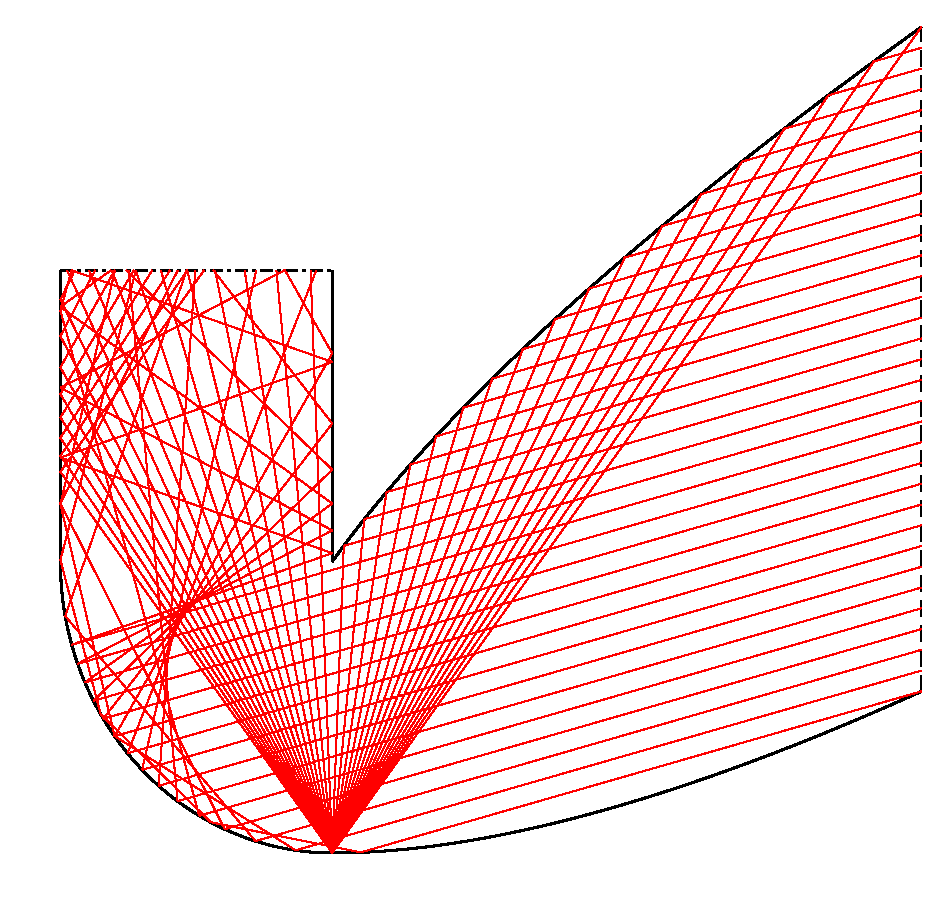
\includegraphics[width=0.90\columnwidth,height=5cm]{figs/2D-diagram-15.eps}
		\subcaption{2D RT diagram at $\rm{a_s = 15^o}$.}
		
		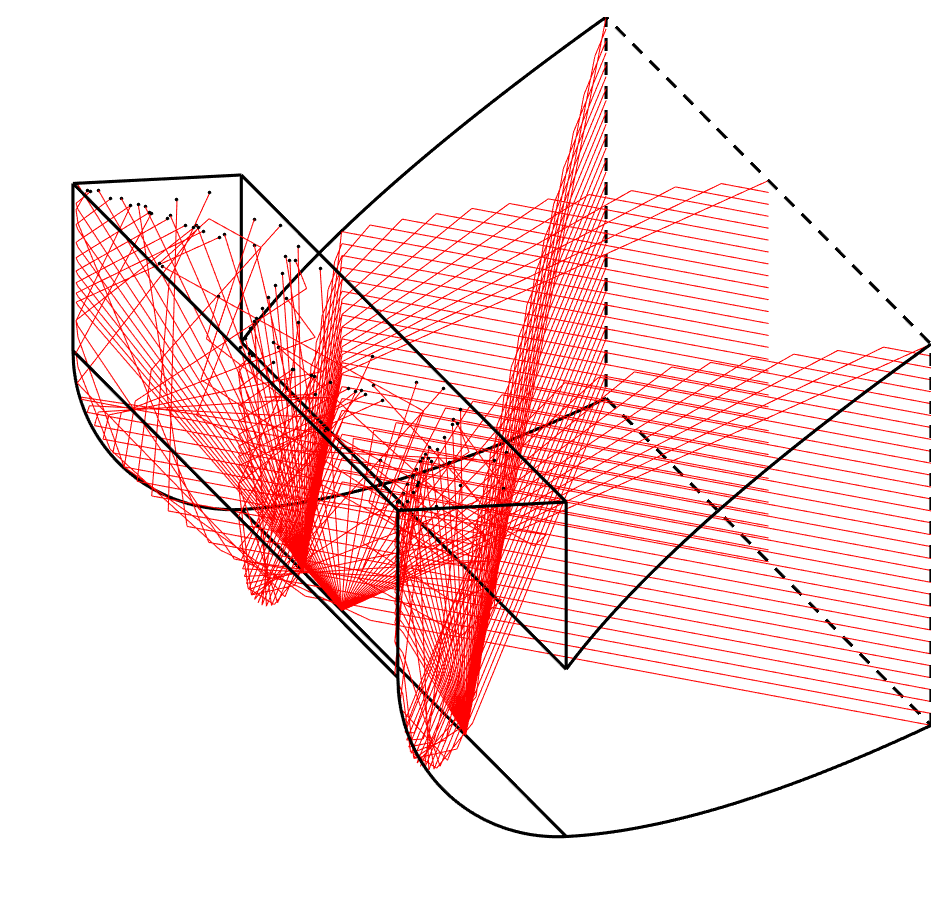
\includegraphics[width=0.95\columnwidth,height=5.5cm]{figs/3D-diagram-15.eps}
		\subcaption{3D RT diagram at $\rm{a_s = 15^o}$ and $\rm{\gamma_s = 70^o}$.}
	\end{minipage}
	\begin{minipage}{0.49\columnwidth}
		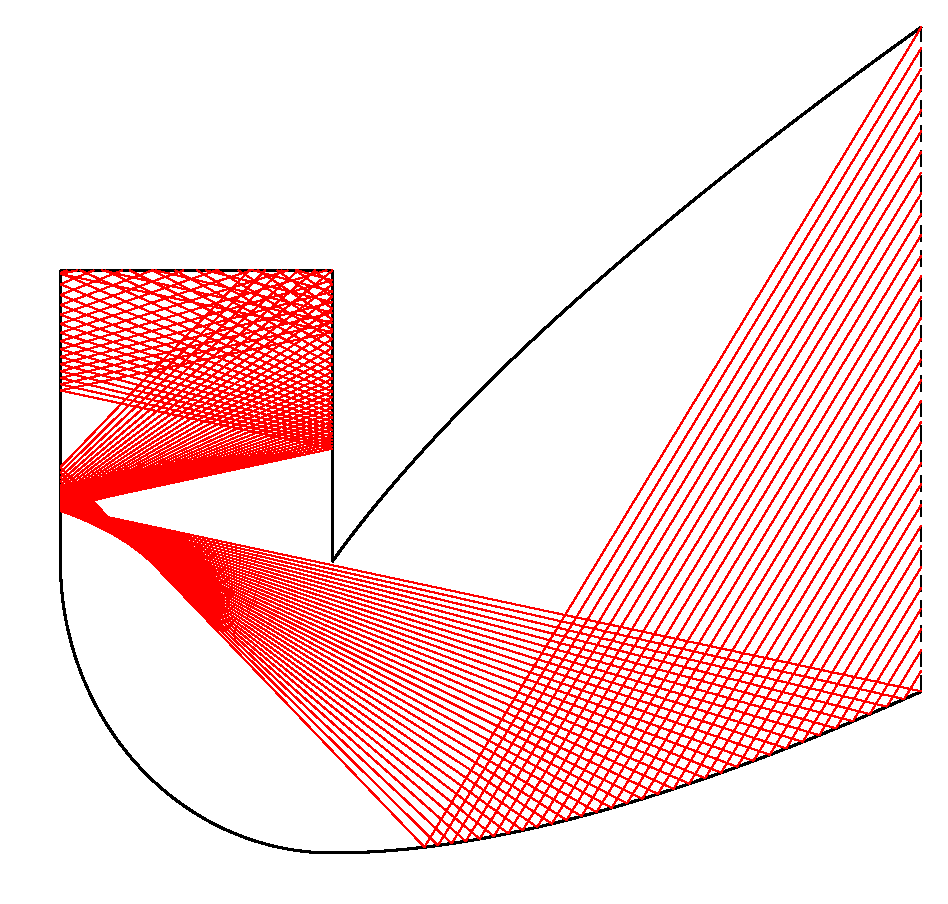
\includegraphics[width=0.90\columnwidth,height=5cm]{figs/2D-diagram-60.eps}
		\subcaption{2D RT diagram at $\rm{a_s = 60^o}$.}
		
		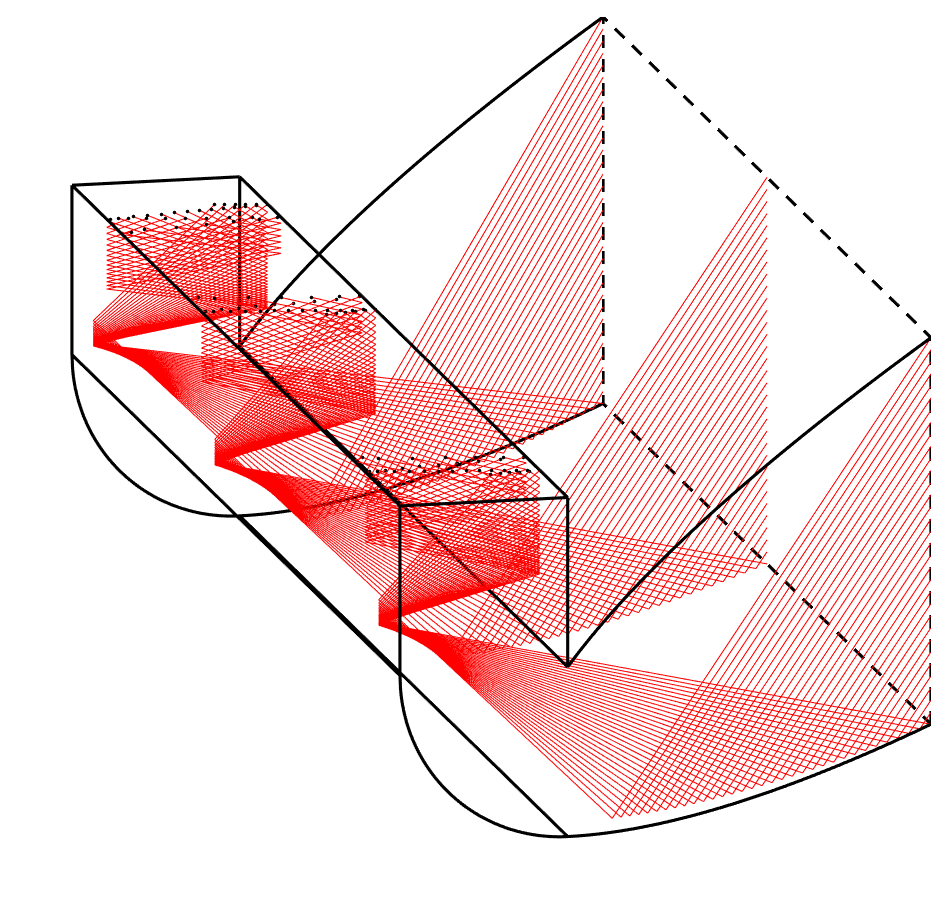
\includegraphics[width=0.95\columnwidth,height=5.5cm]{figs/3D-diagram-60.eps}
		\subcaption{3D RT diagram at $\rm{a_s = 60^o}$ and $\rm{\gamma_s = 10^o}$.}
		
	\end{minipage}
	\caption{Ray tracing diagrams in 2D and 3D.}
	\label{RT-diagram}
\end{figure}

%The glazing transmittance $\tau_{\rm{g}}$, calculated using equations described in \citet{Duffie2013}, is dependent of the inclination $\beta$, which affects the incident angle $\theta_{\rm{i}}$, defined as the angle between the incident solar ray and the normal to the glazing, is calculated by Eq. (\ref{incidence}):
%
%\begin{equation}
%\mathrm{\theta_i = {\cos ^{-1}}\left[ {\cos {a_s}\cos ({\gamma_s} - {\gamma_w})\sin \beta  + \sin {a_s}\cos \beta} \right]}
%\label{incidence}
%\end{equation}
%
%\noindent where $\gamma_{\rm{s}} = 0$ in the 2D analysis, and the concentrator azimuth angle $\gamma_{\rm{w}}$ is zero as the system is south facing.

The optical efficiency is defined as the ratio between the absorbed and the incident solar energy. Considering number of reflections, glazing transmittance and absorber absorptance, it is calculated using Eq. (\ref{optical}) as function of the reflectors' shape and the concentration ratio (\cite{Sellami2013}):

\vspace{-0.75cm}
\begin{equation}
\mathrm{\eta_o = {\mathlarger{\sum\limits}_{\scriptscriptstyle i=1}^{\scriptscriptstyle \mathrm{N_{rays}}}{{\rho_{r}^{{r_i}}}}}\tau_{g}\alpha_{abs}}
\label{optical}
\end{equation}

\noindent where $\rm{r_i}$ is the number of reflections of the solar ray i.

The effective concentration ratio ($\rm{C_{eff}}$), which is the product of the geometric concentration ratio and the optical efficiency, is given by Eq. (\ref{Ceff}). $\rm{C_{eff}}$ is useful to select shapes capable of enhancing both concentration of energy at the absorber and optical efficiency. All the optical outputs $\tau_{\rm g}$, $\eta_{\rm o}$ and $\rm{C_{eff}}$ can be calculated as averaged values to represent the whole period of operation for each particular concentrator. They were referred to as $\tau_{\rm g,avg}$, $\eta_{\rm o,avg}$ and $\rm{C_{eff,avg}}$.

\vspace{-0.75cm}
\begin{equation}
\mathrm{C_{eff} = \eta_{\!_o}CR}
\label{Ceff}
\end{equation}

The collector's dimensions can also be related as dimensionless relative to the absorber width: $\rm{W^{*} = W_{col}/W_{abs}}$, $\rm{H^{*} = H_{col}/W_{abs}}$ and $\rm{L^{*} = L_{col}/W_{abs}}$. The dimensionless parameter A$^*$ was introduced to consider the reflector area relative to the absorber area, where:

\vspace{-0.75cm}
\begin{equation}
\mathrm{{A^*} = \frac{{{A_R}}}{{{A_{abs}}}} = \frac{{{W_r}}}{{{W_{abs}}}} + 2\frac{{{W^*}{H^*}}}{{{L^*}}}}
\label{reflectorarea}
\end{equation}

\noindent where $\rm{W_r}$ is the width of reflective material employed for a particular shape.

\section{Results and Discussion}

\subsection{Overview and collector specification}

This section was organised as follows:

\begin{itemize}[topsep=5pt,partopsep=0pt] \itemsep0pt
\item Design analysis of a standalone collector's geometry by means of the dimensionless parameters W$^{*}$, H$^{*}$ and A$^{*}$ at different parabolic shapes as function of the truncation level (in terms of the geometric concentration ratio CR);
\item Optical performance considering the average values of optical efficiency $\rm{\eta_o}$ and effective concentration ratio $\rm{C_{eff}}$ at different shapes (in terms of $\alpha_{\!_{\rm{P2}}}$) as function of CR at a fixed absorber width, zero tertiary section height ($\rm{H_{TS} = 0}$) and $\rm{L_{col} = 10W_{abs}}$, 
\item Optical performance of two different geometries by varying the length;
\item Selection of the collector for further fabrication;
\item Evaluation of the cavity height on the optical efficiency and the energy distribution over the absorber;
\item Optical characterisation of the collector.
%\item Comparison of the combination of three different concentrator shapes on a fixed area of wall;
%\item Evaluation of the effect of the aperture size of the same collector at a fixed length;
%\item Analysis of different combinations in terms of aperture size at a fixed area of wall.
\end{itemize}

%\subsection{Collector specification}

An optical analysis was conducted for an air heating solar concentrating collector with the following specifications: 

\begin{itemize} [topsep=5pt,partopsep=0pt] \itemsep0pt
    \item The absorber absorptance ($\alpha_{\rm{abs}}$) is 0.85;
    \item The reflector reflectance ($\rho_{\rm{r}}$) is 0.95;
    %\item The absorber surface is placed at the end of the circular section and hence the straight reflectors are not considered;
    \item A 4-mm thick low iron glass was employed with a refractive index of 1.526 and an extinction coefficient of 4 m$^{\!^{-1}}$. When the rays are perpendicular to the surface, the value of $\tau_{\rm{g}}$ is 0.90;
    %\item The glazing inclination $\beta$ was set at 53$^{\circ}$ incurring in the average transmittance of 0.88;
    \item The maximum truncation level was set to result in the minimum geometric concentration ratio of 2.0 regardless of the parabolic shape.
    \item The upper parabola axis angle was set to be coincident to the lowest solar altitude angle ($\alpha_{\!_{\rm{P1}}}$ = 15$^{\circ}$);
    \item The range of lower parabola axis angles ($\alpha_{\!_{\rm{P2}}}$) considered was between 44$^{\circ}$ to 61$^{\circ}$.
\end{itemize}

\subsection{Effect of the glazing inclination on the light transmittance}

Glazing transmittance $\tau_{\rm{g}}$ varies in relation to the incident angle $\theta_{\rm{i}}$ as shown in Figure \ref{transm}.

\Figure[scale=0.52,placement=!ht,label={transm},caption={Transmittance as function of the angle of incidence.}]{figs/transm.eps}

The average transmittance calculated as function of the glazing inclination are shown in Figure \ref{transmittance}. A maximum average transmittance is at \mbox{$\beta$ = 33$^{\circ}$} as 0.8907, thus is the inclination of which the glazing losses are minimum overall. Compared to the transmittance with the glazing placed vertically, there is a relative difference of 14\%. However, an inclination at $\beta$ = 33$^{\circ}$ brings practical difficulties, such as high accumulation of dust and rain water over the glazing cover. For this reason, steeper inclination was desirable, even though there is less solar energy reaching the absorber. Therefore, \mbox{$\beta$ = 62$^{\circ}$} was chosen, where \mbox{$\tau_{\rm{g,avg}}$ = 0.8770}, which is more than 98\% of the maximum average transmittance.

\Figure[scale=0.55,placement=!ht,label={transmittance},caption={Average transmittance dependent on glazing inclination.}]{figs/transmittance.eps}

The results of instantaneous light transmittance against daytime is shown in Figure \ref{transm-time} for different glazing inclinations on 30$^{\rm th}$ June. The maximum transmittance profile is at $\beta$ = 33$^{\circ}$, whereas the one of inclination at the local latitude angle ($\beta$ = 53$^{\circ}$) and the one at $\beta$ = 62$^{\circ}$ do not present significant difference. All the three profiles are similar between 11h and 16h of this day. On the other hand, the profile of which the glazing is at the vertical shows the highest amount of solar reflection.

\Figure[scale=0.50,placement=!ht,label={transm-time},caption={Light transmittance throughout the day (30$^{\rm th}$ June).}]{figs/transm-time.eps}

\subsection{Design analysis of standalone collectors}

The dimensionless parameters $\rm{W^{*}}$ and $\rm{H^{*}}$ are presented by graphs in Figure \ref{size_region2}, where each graph corresponds to a particular shape. The maximum concentration ratio, obtained from the shape at $\theta_{\!_{\rm{P2}}} = 44^{\circ}$, was found to be 2.98. For the same concentration ratio, both $\rm{W^{*}}$ and $\rm{H^{*}}$ decrease as $\theta_{\!_{\rm{P2}}}$ increases because the concentrator's acceptance angle is broader. For the same concentrator (fixed shape), the size increases when CR also increases until its maximum aperture width, thus defining its maximum size (indicated by the dashed line in Figure \ref{size_region2}). The smallest concentrator has the shape of narrowest acceptance angle ($\theta_{\!_{\rm{P2}}} = 44^{\circ}$) and smallest concentration ratio (CR = 2.0) for being the most truncated ($\rm{W_{col} = 2.2W_{abs}}$ and $\rm{H_{col} = 2.2W_{abs}}$), whereas the largest concentrator has also the narrowest acceptance angle but at the highest concentration ratio ($\rm{W_{col} = 7.3W_{abs}}$ and $\rm{H_{col} = 5.4W_{abs}}$). 

As shown in Figure \ref{reflector_region}, the dimensionless parameter $\rm{A^{*}}$ increases as the concentrator's size increases. Thus the graphs in Figures \ref{size_region2} and \ref{reflector_region} are similar. The reflector area varied from $\rm{5.4A_{abs}}$ for the smallest concentrator to nearly $\rm{24A_{abs}}$ for the largest one. Because this collector is an asymmetric compound parabolic concentrator, these graphs are similar to those found by \citet{Rabl1976} for symmetric concentrators.

\Figure[scale=0.70,placement=!ht,label={size_region2},caption={Dimensionless parameters $\rm{W^{*}}$ and $\rm{H^{*}}$ matching particular CR for different shapes.}]{figs/size_region2.eps}

\Figure[scale=0.70,placement=!ht,label={reflector_region},caption={Dimensionless parameter $\rm{A^{*}}$ matching particular CR for different shapes.}]{figs/reflector_region.eps}

\Figure[scale=0.80,placement=!ht,label={size_region3},caption={Dimensionless parameter $\rm{A^{*}}$ matching particular CR for different shapes.}]{figs/size_region3.eps}

\subsection{Optical performance of standalone collectors}

\subsubsection{Optical performance by varying parabolic shape and truncation level}

The average optical efficiency as a function of CR for different shapes are shown in Figure \ref{eff_region2}. For concentrators of concentration ratio below 2.2 the shape of highest optical efficiency is the one of $\theta_{\!_{\rm{P2}}} = 44^{\circ}$. For truncation levels resulting in concentration ratio above 2.4, concentrators are unable to accept a portion of direct solar radiation of solar altitude angles ($\rm{a_s}$) above 50$^{\circ}$, which is the reason why the graphs has decaying behaviours. The shape of $\theta_{\!_{\rm{P2}}} = 44^{\circ}$ and CR = 2.0 is the most efficient with $\rm{\eta_{o,avg} = 0.689}$ for being the smallest concentrator that accepts all direct solar radiation in the period of operation. The least efficient concentrator is the one of maximum CR ($\rm{\eta_{o,avg} = 0.432}$) because it requires more reflections for the solar rays to reach the absorber and it does not accept direct solar radiation above $\rm{50^{\circ}}$ of $\rm{a_s}$, which is equivalent to 35\% of the period of operation.

\Figure[scale=0.7,placement=!ht,label={eff_region2},caption={$\rm{\eta_{o,avg}}$ matching particular CR for different shapes.}]{figs/eff_region2.eps}

The average effective concentration ratio $\rm{C_{eff,avg}}$ against CR and $\theta_{\!_{\rm{P2}}}$ is shown in Figure \ref{Ceff_region2}. Geometries of $\theta_{\!_{\rm{P2}}}$ below 56$^{\circ}$ have maximum values of $\rm{C_{eff,avg}}$ above 1.55 at each particular level of CR. After these conditions, the graphs drop dramatically as CR is increased due to the optical efficiency fall discussed previously. The shape correspondent to the smallest $\rm{C_{eff,avg}}$ is the one of maximum CR ($\rm{C_{eff,avg} = 1.3}$) for being the least optically efficient; and the shape of maximum $\rm{C_{eff,avg}}$ is the one of $\theta_{\!_{\rm{P2}}} = 51^{\circ}$ and $\rm{CR = 2.5}$ although it is not able to accept direct solar radiation above $\rm{56^{\circ}}$ of $\rm{a_s}$. Concentrators of $\rm{CR = 2.0}$ are less effective in $\rm{C_{eff,avg}}$ despite being the most optically efficient concentrators.

\Figure[scale=0.7,placement=!ht,label={Ceff_region2},caption={$\rm{C_{eff,avg}}$ matching particular CR for different shapes.}]{figs/Ceff_region2.eps}

\subsubsection{Optical performance by varying concentrator length} 

The values of ${\rm \eta_{o,avg}}$ and $\rm{C_{eff,avg}}$ were calculated as function of the dimensionless parameter $\rm{L^{*}}$ for two different concentrators: the most optically efficient (CR = 2.0) and one with highest $\rm{C_{eff,avg}}$ (CR = 2.5). The results can be seen in Figure \ref{eff_length}. The values of ${\rm \eta_{o,avg}}$ assuming an infinite length were found to be 0.70 (CR = 2.0) and 0.662 (CR = 2.5). The end losses are higher for shorter concentrators due to greater number of reflections. When length equals 3$\rm W_{abs}$, where $\rm \eta_{o,avg}$ is more than 95\% of the optical efficiency assuming infinite length. When $\rm{L_{col} = 10W_{abs}}$, the values of $\rm{\eta_{o,avg}}$ are more than 98\% of those assuming infinite length. Hence, longer concentrator incurs in less reflections losses at the ends, thus leading to higher optical efficiencies. However the cost of additional reflective material and weight might not compensate the little significant gain in energy collection.

\Figure[scale=0.75,placement=!ht,label={eff_length},caption={${\rm \eta_{o,avg}}$ matching particular $\rm{L^{*}}$ for two different concentrators.}]{figs/eff_length.eps}

The end effect can be observed in more details when ${\rm \eta_{o,avg}}$ for five different length ratios are plotted against time of operation. This is shown in Figure \ref{length_variance} specifically on 30$^{\rm th}$ of June for the smallest concentrator's performance (CR = 2.0). The end losses are higher in the beginning of the day due to higher values of the azimuth solar angles $\gamma_{\rm s}$ incurring in more reflections at the ends and therefore collectors collect less energy before noon, especially for shorter concentrators. 

\Figure[scale=0.70,placement=!ht,label={length_variance},caption={${\rm \eta_o}$ vs. time for a collector at different length ratios.}]{figs/length_variance.eps}

\subsection{Selection of the collector to be fabricated}

In this topic, a criterion was used to select the collector's geometry to be fabricated for tests. As mentioned in section 3.3, the collector must accept direct solar radiation with altitude solar angles between 15$^{\circ}$ and 61$^{\circ}$. Once these limits are set, an initial design of the collector was sketched of which the angles of both parabolic axes are coincident to those limits so that all direct radiation within this range is accepted. From the initial design (shown in Figure \ref{collectors-61-50} in red), the absorber width was found with the aim of achieving the maximum concentration ratio, which is 2.284. The actual aperture width ($\rm{W_{apt}}$) will be 330 mm in order to have three collectors stacked on every metre of wall height. Hence, the absorber width ($\rm{W_{abs}}$) was calculated and found to be 145 mm.

\Figure[scale=0.70,placement=!ht,label={collectors-61-50},caption={Comparison between the collector at 61$^{\circ}$ of $\theta_{\!_{\rm{P2}}}$ (red) and the one at 50$^{\circ}$ of $\theta_{\!_{\rm{P2}}}$ (blue).}]{figs/collectors-61-50.eps}

As this collector is truncated, the range of angular acceptance may be broader than the limits previously defined. In order to validate this hypothesis, the ray tracing algorithm was used to check whether all the rays within this range are accepted. A graph of $\theta_{\rm{acc}}$ vs. ${\rm{a_s}}$ was plotted and shown in Figure \ref{acceptance}. The collector fully accepts direct radiation from 17$^{\circ}$ to 63$^{\circ}$ of ${\rm{a_s}}$, which exceeds the upper limit. Therefore, the collector's optical performance can be enhanced by further modifications to the reflectors. In this particular case, it was done by decreasing the lower parabola axis angle ($\theta_{\!_{\rm{P2}}}$). As this change in shape affects the number of reflections, $\rm{\eta_{\!_{o,avg}}}$ was calculated at different values of $\theta_{\!_{\rm{P2}}}$ and two graphs were plotted in Figure \ref{eff-alphaP2}. Although there is no significant gain in the average effective concentration ratio ($\rm{C_{eff,avg}}$ = 1.52) when both designs are compared, the parameter A* is reduced from 11.7 to 7.8, hence reducing the reflector area required by 33\%.

%Embora não haja um ganho significativo na average effective concentration ratio (Ceff,avg = 1.52) quando se compara ambos os designs, o valor de A* caiu de 11.7 para 7.8, reduzindo a quantidade de área de refletor em 33\%.

\Figure[scale=0.70,placement=!ht,label={acceptance},caption={Angular acceptance vs. solar altitude angle for the collector at 61$^{\circ}$ of $\alpha_{\!_{\rm{P2}}}$ (red) and the one at 50$^{\circ}$ of $\alpha_{\!_{\rm{P2}}}$ (blue).}]{figs/acceptance-graph.eps}

Furthermore, by ray tracing, the collector's angular acceptance at \mbox{$\theta_{\!_{\rm{P2}}}$ = 50$^{\circ}$} was calculated and shown in Figure \ref{acceptance} (in red). Although the full acceptance is up to 59$^{\circ}$, $\rm{\theta_{acc}}$ at 60$^{\circ}$ is above 90\%, which poorly influences the optical efficiency. From this analysis, the angles of the upper and lower parabola axes was chosen to be 17$^{\rm o}$ and 50$^{\rm o}$ respectively. 

\Figure[scale=0.70,placement=!ht,label={eff-alphaP2},caption={Average optical efficiency {\itshape versus} lower parabola axis angle.}]{figs/eff-alphaP2.eps}



%para a escolha do comprimento do coletor, utilizou-se ray tracing para obter os valores de eta0avg em função deste parametro geometrico. o gráfico de eta0,avg x Lcol foi plotado e mostrado na figura 3.23. para comprimentos maiores que 2 m, nao há ganho significativo de eficiencia. Para comprimentos menores que este valor, as perdas por reflexao nas laterais se intensificam, o que não favorece no rendimento ótico do coletor. Para o comprimento de 1.25 m, sua eficiencia ótica está a 90\% da eficiência máxima teórica. Então pelo ponto de vista ótico, este comprimento foi escolhido para a fabricaçao do coletor.

For the selection of the collector's length, ray tracing technique was used to calculate the average optical efficiency as function of this geometric parameter. The graph of $\rm{\eta_{\!_{o,avg}}}$ versus $\rm{L_{col}}$ was plotted and shown in Figure \ref{eff-length}. For lengths above 2 m, there is little gain in efficiency (above 0.68), whereas below this value, the reflection losses at the ends are higher, which worsens the optical performance. At $\rm{L_{col}}$ = 1.25 m, the collector's optical efficiency is 95\% of the maximum theoretical efficiency ($\rm{\eta_{\!_{o,avg}}}$ = 0.67). Therefore, under the optical consideration, this length was chosen for the collector's fabrication.

\Figure[scale=0.70,placement=!ht,label={eff-length},caption={Average optical efficiency {\itshape versus} collector's length.}]{figs/eff-length.eps}

\section{Optical characterisation of the proposed collector}

\subsection{Effect of the cavity height}

To understand the effect of the cavity height in the analysis, the average optical efficiency was calculated and shown in Figure \ref{opt-avg-hts} as function of the tertiary section height. These results are straightforward, as the addition of a new reflective section will imply in more reflections, thus decreasing the average efficiency by approximately 3.5\%.

\Figure[scale=0.70,placement=!ht,label={opt-avg-hts},caption={Average optical efficiency as function of the tertiary section height.}]{figs/opt-avg-hts.eps}

To better illustrate the effect of the tertiary section height, the optical profile of the collector on 30$^{\rm th}$ of June at three different heights was calculated and shown in Figure \ref{opt-eff-3hts}. From 09:00 to 10:30 and from 16:20 to 17:00 the three profiles impose nearly the same efficiency. The highest difference is at 12:00, where $\eta_{\rm{o}}$ with no tertiary height is 0.71 and $\eta_{\rm{o}}$ at $\rm{H_{TS}}$ = $\rm{W_{abs}}$ is 0.61.

\Figure[scale=0.70,placement=!ht,label={opt-eff-3hts},caption={Optical efficiency profile for three tertiary section heights on 30$^{\rm th}$ of June.}]{figs/opt-eff-3hts.eps}

Although the optical efficiency is reduced by the increase of the tertiary section height, the cavity has a function of distributing the incoming energy uniformly along the absorber surface. To apply this function, the results of the simulation ${\rm{a_s}}$ at 54$^{\circ}$ was selected as an example and this can be seen in Figures \ref{Tertiary-hts0}, \ref{Tertiary-hts72} and \ref{Tertiary-hts145}. From Figure \ref{Tertiary-hts0}, a high energy peak concentrated in one millimetre of absorber width is observed (12500 W/m$^2$) and all the energy is concentrated in 45 millimetres. From Figure \ref{Tertiary-hts72} the energy flux is distributed through all the absorber area where the peak region of 980 W/m$^2$ is concentrated in 6 mm of width. From Figure \ref{Tertiary-hts145}, the energy is more distributed across the absorber surface, where the maximum energy flux is 740 W/m$^2$ across half the absorber width. Hence, the tertiary section helps to distribute the solar energy more uniformly over the absorber area, which is desirable for further heat transfer even though the reflection losses are higher. For this reason, the cavity height was set to be 145 mm.

\begin{figure}[ht!]
	\begin{minipage}{0.48\columnwidth}
		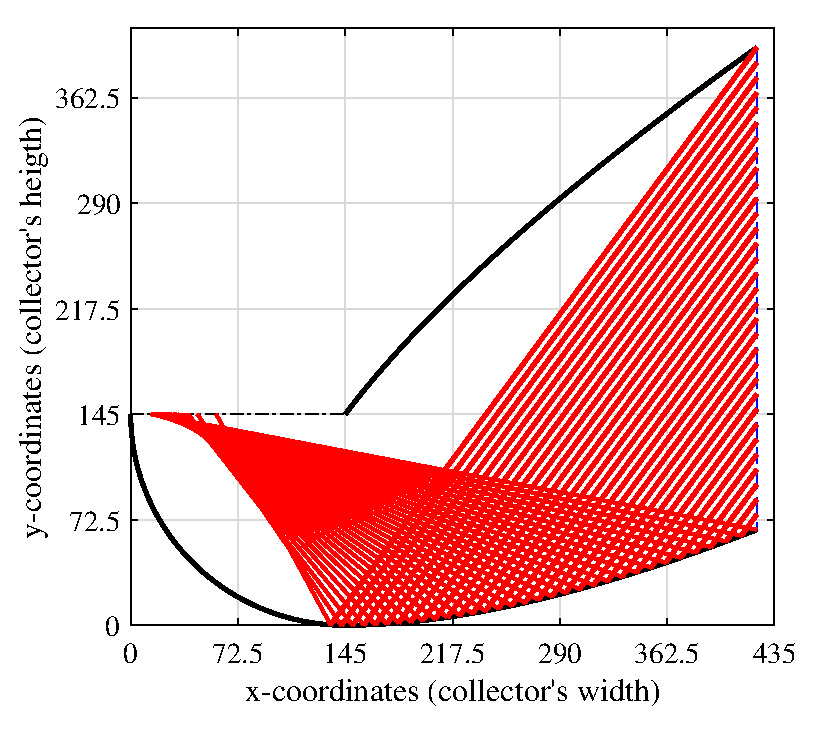
\includegraphics[scale=0.48]{figs/RT2D-hts0.eps}
		\subcaption{Ray tracing diagram (cross section).}
		
	\end{minipage}
	\begin{minipage}{0.48\columnwidth}
		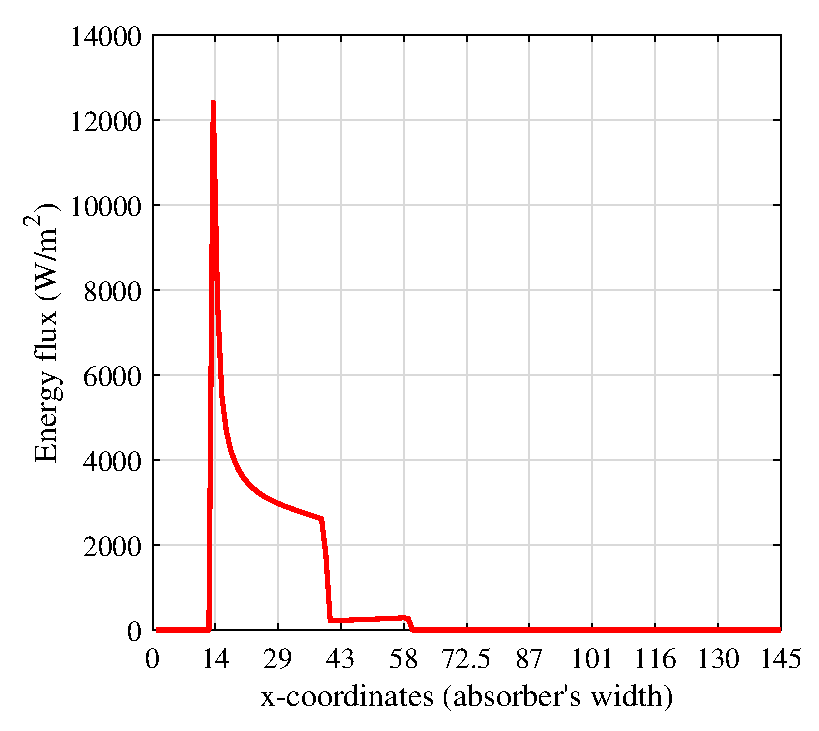
\includegraphics[scale=0.48]{figs/Energy2D-hts0.eps}
		%\\[-9mm]
		\subcaption{Energy flux distribution (cross section).}
	\end{minipage}
\\[3mm]
	\begin{minipage}{1.0\columnwidth}
	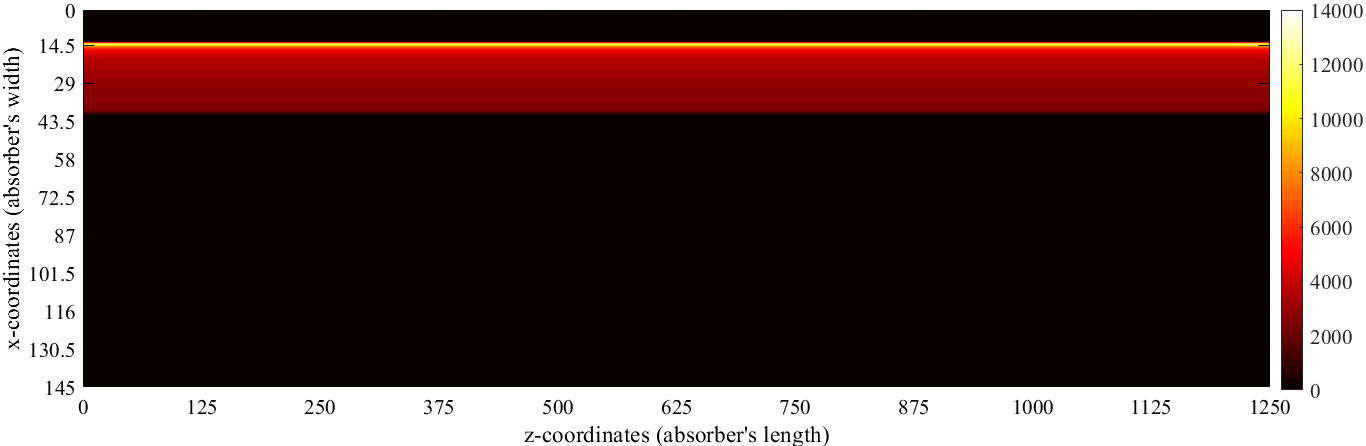
\includegraphics[scale=0.41]{figs/Energy3D-hts0.png}
	\subcaption{Energy flux distribution over the absorber surface (top view).}
	\end{minipage}

	\caption{Ray tracing diagram in 2D and energy flux distribution over the absorber width with no tertiary section.}
	\label{Tertiary-hts0}
\end{figure}

\begin{figure}[ht!]
	\begin{minipage}{0.48\columnwidth}
		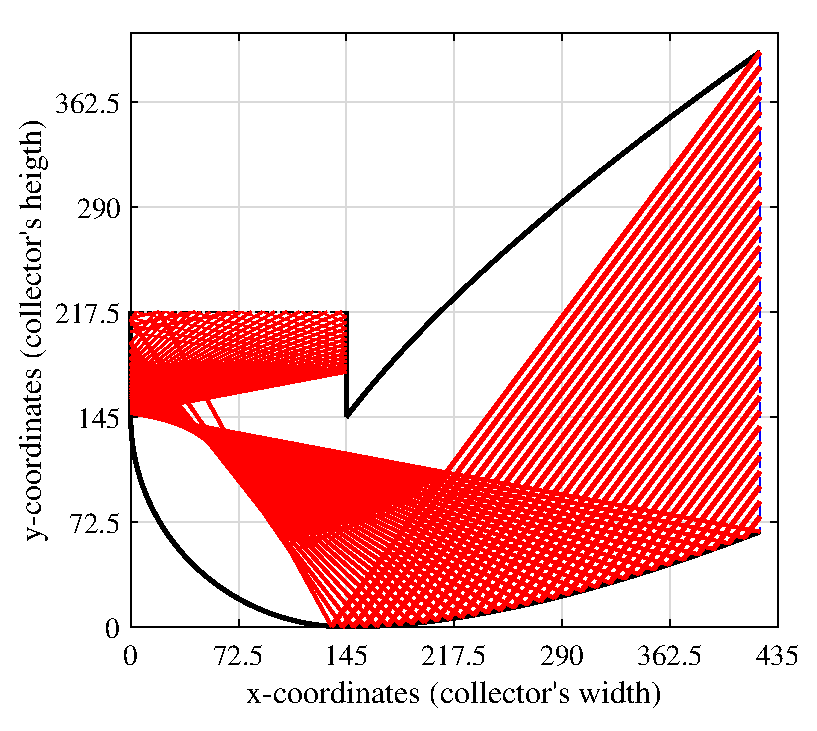
\includegraphics[scale=0.48]{figs/RT2D-hts72.eps}
		\subcaption{Ray tracing diagram (cross section).}
		
	\end{minipage}
	\begin{minipage}{0.48\columnwidth}
		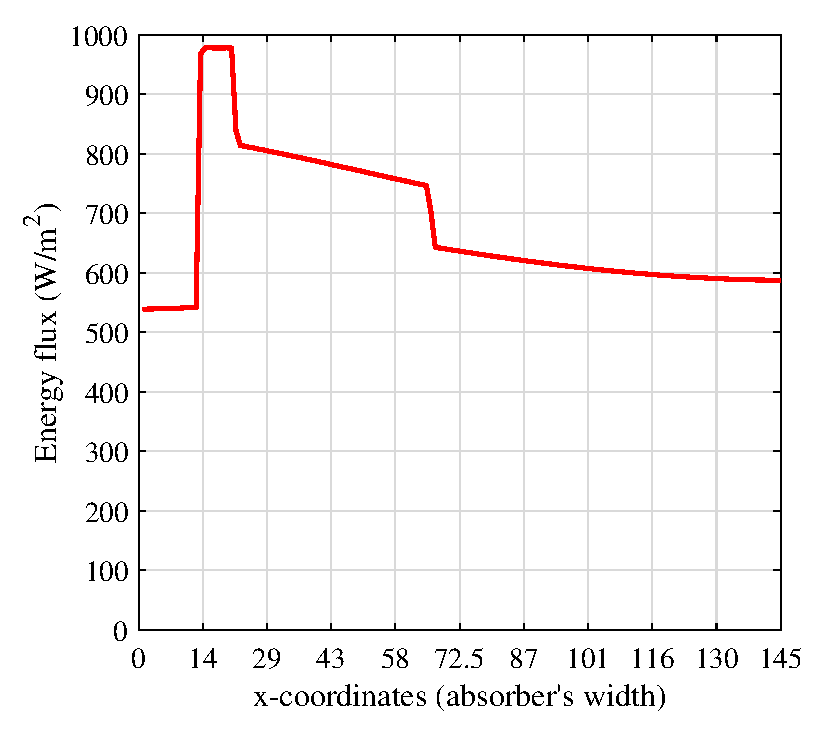
\includegraphics[scale=0.48]{figs/Energy2D-hts72.eps}
		%\\[-9mm]
		\subcaption{Energy flux distribution (cross section).}
	\end{minipage}
	\\[3mm]
	\begin{minipage}{1.0\columnwidth}
		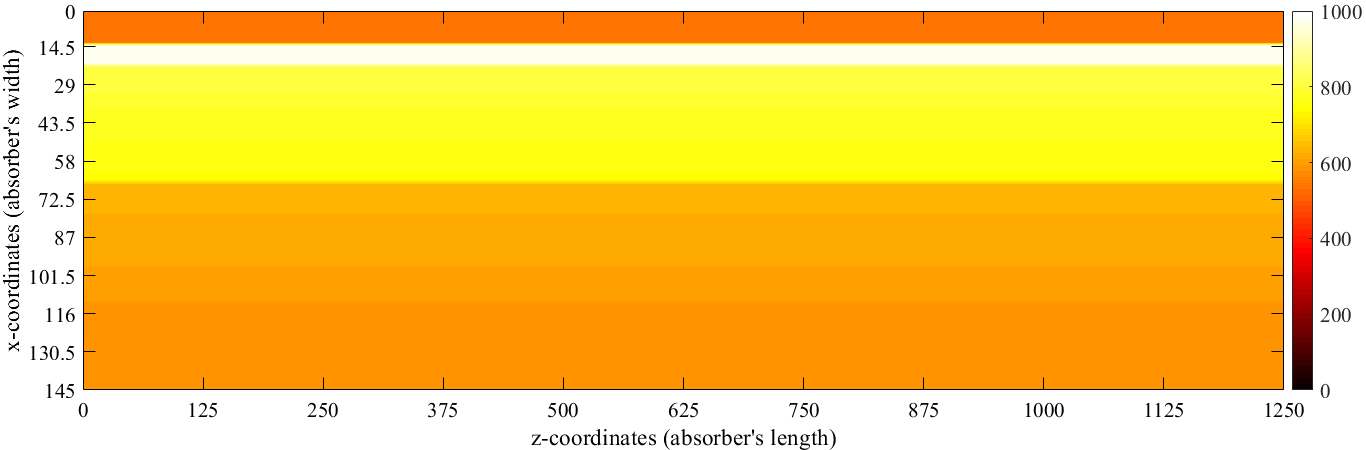
\includegraphics[scale=0.41]{figs/Energy3D-hts72.png}
		\subcaption{Energy flux distribution over the absorber surface (top view).}
	\end{minipage}
	
	\caption{Ray tracing diagram in 2D and energy flux distribution over the absorber width with tertiary section height of 72.5 mm.}
	\label{Tertiary-hts72}
\end{figure}

\begin{figure}[ht!]
	\begin{minipage}{0.48\columnwidth}
		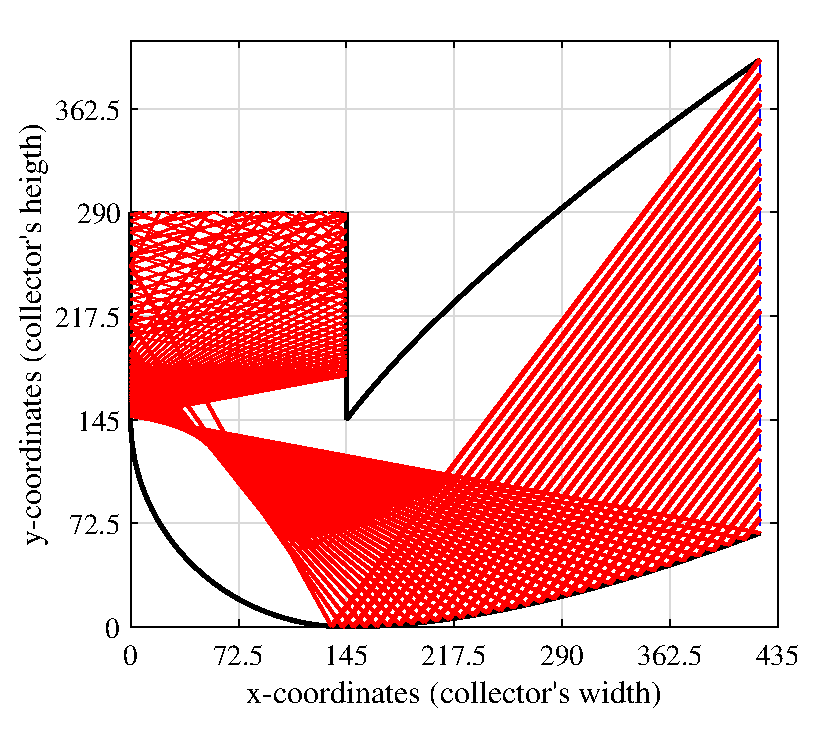
\includegraphics[scale=0.48]{figs/RT2D-hts145.eps}
		\subcaption{Ray tracing diagram (cross section).}
		
	\end{minipage}
	\begin{minipage}{0.48\columnwidth}
		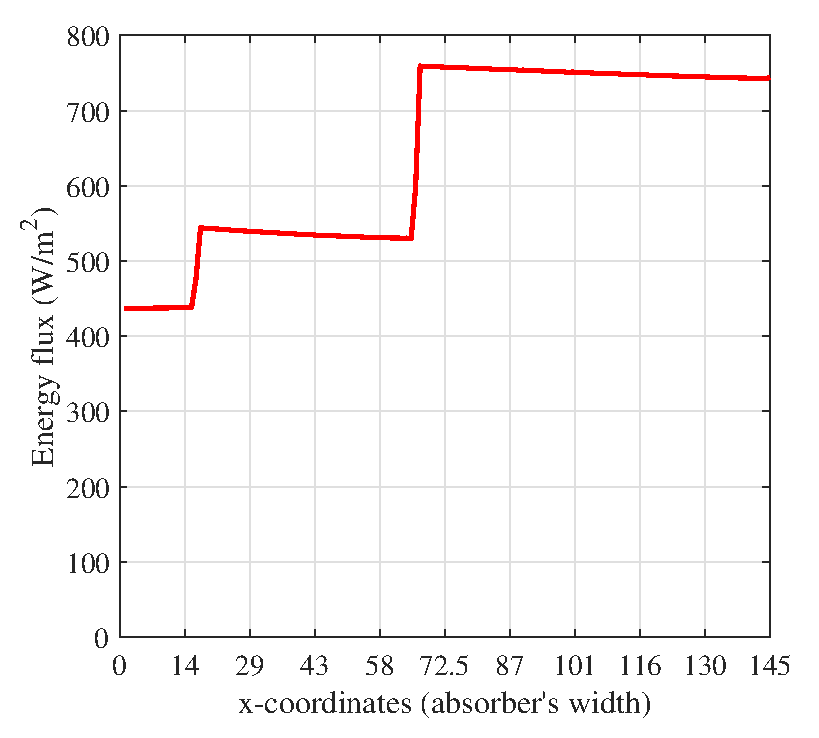
\includegraphics[scale=0.48]{figs/Energy2D-hts145.eps}
		%\\[-9mm]
		\subcaption{Energy flux distribution (cross section).}
	\end{minipage}
	\\[3mm]
	\begin{minipage}{1.0\columnwidth}
		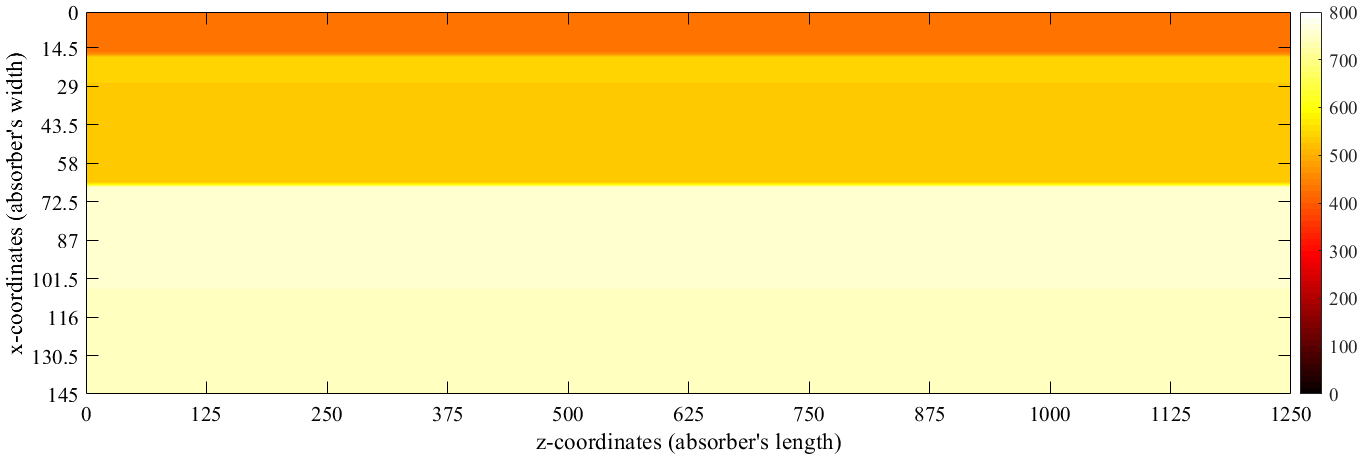
\includegraphics[scale=0.41]{figs/Energy3D-hts145.png}
		\subcaption{Energy flux distribution over the absorber surface (top view).}
	\end{minipage}
	
	\caption{Ray tracing diagram in 2D and energy flux distribution over the absorber width with tertiary section height of 145 mm.}
	\label{Tertiary-hts145}
\end{figure}

\subsection{Optical efficiency profile}

After the optical analysis, the concentrator's design has been defined as shown in Figure \ref{collector3p} and the main geometric parameters are summarised in Table \ref{optics_parameters}. The glazing inclination has been set at $\beta$ = 62$^{\circ}$ due to practical reasons related to its width. 
%Moreover, Figure \ref{reflector1} shows a system of three collectors stacked on the wall.

\Figure[scale=0.75,placement=!ht,label={collector3p},caption={Cross section of the collector's final design.}]{figs/collector3p.eps}

\begin{table}[!ht]
	\caption{Geometric parameters of the concentrator to be fabricated.}
	\centering
	\begin{tabular}{p{1.75cm}p{4.5cm}p{2.0cm}}
		\hline \\[-10pt]
		Symbol & Geometric parameter & Value \\ [2pt]
		\hline \\[-12pt]
		$\rm{L_{col}}$ & Concentrator length & 1.25 m \\ [2pt]
		
		$\rm{H_{col}}$ & Concentrator height & 0.40 m \\ [2pt]
		
		$\rm{W_{col}}$ & Concentrator depth & 0.43 m \\ [2pt]
		
		$\rm{W_{abs}}$ & Absorber width & 0.145 m \\ [2pt]
		
		$\rm{A_{abs}}$ & Absorber area & 0.18 m$^2$ \\ [2pt]
		
		$\rm{W_{glaz}}$ & Glazing width & 0.27 m \\ [2pt]
		
		$\rm{A_{glaz}}$ & Glazing area & 0.34 m$^2$ \\ [2pt]
		
		$\beta$ & Glazing inclination & 62$^{\circ}$ \\ [2pt]
		
		$\rm{W_{apt}}$ & Aperture width & 0.33 m \\ [2pt]
		
		$\rm{A_{apt}}$ & Aperture area & 0.41 m$^2$ \\ [2pt]
		
		$\rm{H_{\!_{TS}}}$ & Cavity height & 0.145 m \\ [2pt]
		
		$\rm{CR}$ & Concentration ratio & 2.28 \\ [2pt]
		
		$\rm{A_{R}}$ & Reflector area & 2 m$^2$ \\
		
		\hline 
	\end{tabular}
	\label{optics_parameters}
\end{table}

It is also important to show the optical profile as in Figure \ref{opt-eff-time}, where the optical efficiency is presented as function of daytime and date during the summer. At early in the morning, the optical efficiency is lower due to larger number of reflections at one end of the collector and from 10:30 the efficiency keeps higher than 0.60 and the maximum value is 0.69 at noon one the last days of summer. The average optical efficiency for direct radiation of this collector is 0.67. It is worth noting that the optical profiles of multiple stacked collectors operating in connection are identical, which results in an equivalent quantity of energy available on the absorber surface in each collector. To determine the amount of energy absorbed by a flow of air, it is imperative to conduct experimental studies or utilize a valid energy balance calculation.

\Figure[scale=0.70,placement=!ht,label={opt-eff-time},caption={Optical efficiency profile throughout the whole period of operation.}]{figs/opt-eff-time.eps}

\section{Chapter Summary}

The selection of an air heater concentrator with the absorber horizontally facing downwards aims to concentrate solar thermal energy inside the cavity and suppress heat losses. With the assistance of a ray tracing technique in 3D, an optical analysis has been undertaken to evaluate its optical efficiency considering factors as: glazing transmittance, truncation level, length and tertiary section height. The results show that there is a maximum value of optical efficiency for a particular parabolic reflector shape and a maximum value of glazing transmittance at different inclinations. It was also concluded that the energy distributed along the absorber area is more uniform with a tertiary section rather than without it even though the optical losses are higher. The effect of the tertiary section on the collector's performance needs to be further assessed, via thermal modelling and outdoor experiments. Finally, a solar concentrator design was proposed through optical analysis, and its 3D optical profile over time was presented at the end of the chapter. The proposed air heater concentrator is able to absorb in average 67\% of direct solar radiation during most part of the day in the period evaluated.

%\Figure[scale=0.85,placement=!ht,label={reflector1},caption={Building integrated stacked system with three concentrators of 0.33 m in aperture width and 1.25 m in length.}]{figs/assembly2.png}

%\section{Future Work}
%
%The next work in optical analysis to be developed are to:
%
%\begin{itemize}
%	\item Present the energy distribution using the ray tracing in 3D;
%	\item Perform a 3D analysis regarding the length of the concentrator;
%	\item Undertake the optical analysis for more than one collector.
%\end{itemize}


%\begin{itemize}[topsep=5pt,partopsep=0pt] \itemsep0pt
%\item {\bf Primary section \ding{172}:} This consists of the aperture and two asymmetric parabolic reflective surfaces. These reflectors are responsible for reflecting solar rays coming through the aperture and concentrate them to the next section;
%\item {\bf Secondary section \ding{173}:} This comprises a circular reflector, whose radius is the absorber width, that reflects all the incoming rays upwards towards the tertiary section;
%\item {\bf Tertiary section \ding{174}:} This consists of a cavity composed of two vertically straight reflectors that receives the solar rays from the secondary section and directs them to the absorber surface. %This section also has a function of keeping the convection suppressed at the absorber due to the formation of a thermally stratified air layer within the cavity (\cite{Norton1991}).
%\end{itemize}

%\begin{description}[topsep=5pt,partopsep=0pt] \itemsep0pt
%    \item [Aperture position:] The concentrator's aperture is set at the vertical position (at the truncation line in Figure \ref{CSview}) so that shading can be avoided when two or more collectors are stacked on a vertical wall enabling the full fa\c{c}ade area available to be harnessed;
%    \item [Parabolic shape:] The angles of both parabolas axes ($\theta_{\!_{\rm{P1}}}$ and $\theta_{\!_{\rm{P2}}}$) define the parabolic shape, therefore affecting size, angular acceptance range (\cite{Zacharopoulos2000}; \cite{Harmim2012}) and maximum geometric concentration ratio (\cite{Mills1978}). Given the same level of concentration ratio, concentrators of narrow angular acceptance are more efficient so collect higher amounts of the available solar energy (\cite{Sarmah2011});
%    \item [Truncation level:] Truncation is an effective way to reduce reflector costs and collector's size. The effect of this on concentration ratio, height-aperture width ratio and reflector length has been studied extensively (\cite{Rabl1976}; \cite{McIntire1979}). Truncated concentrators accept solar rays at broader incident angles due to reduction of reflections, then more of the available solar energy is collected (\cite{Carvalho1985}).;
%    \item [Length and end effect:] If a linear concentrator is long in east-west orientation compared to its width and height, it can be assumed to behave as a two dimensional system where end effects are negligible (\cite{Eames1993a}). For concentrators with short axial lengths, the end losses need to be included on the optical analysis as a portion of reflected solar rays may not reach the absorber under certain obtuse solar incident angles. End loss factors dependent on the incident angle have been analytically calculated for imaging parabolic troughs (\cite{Rabl1985}) and for linear Fresnel concentrators (\cite{Pu2011}; \cite{Heimsath2014}; \cite{Hongn2015});
%    \item [Glazing position:] The glazing placed from the aperture confines heated air in the collectors, as well as offering protection for the collector interior against weather conditions (\cite{Shams2016}). Its position at a given inclination $\beta$ seeks to gain solar energy transmittance.
%    \item [Cavity height:] The cavity contributes to the formation of thermally stratified air layers below the absorber that suppresses convective and radiative heat losses. The height of this cavity affects the distribution of incoming solar radiation along the absorber surface in a way to enhance heat transfer mechanism and mitigate hot spots.
%\end{description}


%The absorber surface is inverted to reduce radiation loss and stabilise the thermal layers below, which improves the heat transfer mechanism. Additionally, it is perforated to allow the airflow to percolate through the holes, thus enhancing the heat transferred from the absorber (\cite{Shams2016}).

%The concentrator's aperture is set at the vertical position (at the truncation line indicated in Figure \ref{CSview}) so that shading can be avoided when two or more collectors are stacked on a wall. The actual aperture width ($\rm{W_{apt}}$) will be 330 mm in order to have three collectors stacked on every metre of wall height. The glazing placed in the primary section works as a heat trap, as well as offering protection for the interior of the unit against weather conditions. Its position at a given inclination $\beta$ seeks to maximise light transmittance over the operation period considered.

%Considerations have also been given to the angles of both parabolas axes ($\alpha_{\!_{\rm{P1}}}$ and $\alpha_{\!_{\rm{P2}}}$), which influence the primary section shape. Those angles also determine the range of solar altitude angle accepted by the system (\cite{Zacharopoulos2000}). The selection of all these design variables must take into account the compromise between optical efficiency and geometric concentration ratio to maximise solar radiation collection at the absorber surface.


%and can be expressed as:
%\begin{equation}
%\mathrm{{\delta_s} = 23.45\sin \left[ {\frac{{360}}{{365}}\left( %{284 + n} \right)} \right]}
%\label{dec}
%\end{equation}


%\begin{description}[topsep=5pt,partopsep=0pt] \itemsep0pt
%	\item[Upper reflector:] $\rm{{W_{abs}} \le {x} \le {x_{apt}}}$ and $\rm{{W_{abs}} \le {y} \le {y_{apt,upper}}}$
%	\item[Lower reflector:] $\rm{{W_{abs}} \le {x} \le {x_{apt}}}$ and $\rm{0 \le {y} \le {y_{apt,lower}}}$
%\end{description}

%They were obtained using basic geometry and SolidWorks$^{\circledR}$. %After applying the transformation, both parabolas were plotted as shown in Figure \ref{rottrans_two}.

%\Figure[scale=0.62,placement=!ht,label={rottrans_two},caption={Parabolas at the initial position (dashed line) and after Affine technique (full line) for the (a) upper and (b) lower parabolas.}]{figs/rottrans_two.png}

%\Figure[scale=0.70,placement=!ht,label={rottrans_upper},caption={Representation of the circular section of central point ($W_{abs}$, $W_{abs}$) and radius $W_{abs}$.}]{figs/rottrans_upper.png}

%\Figure[scale=0.80,placement=!ht,label={rottrans_lower},caption={Representation of the circular section of central point ($W_{abs}$, $W_{abs}$) and radius $W_{abs}$.}]{figs/rottrans_lower.png}

%\Figure[scale=0.55,placement=!ht,label={twoparabolas2},caption={Truncated primary section (ABCD), where AC and BD are the upper and lower reflectors, respectively.},shortcaption={Truncated primary section (ABCD)}]{figs/twoparabolas2.eps}

%\Figure[scale=0.60,placement=!ht,label={quarter_circle},caption={Circular reflector drawing with centre ($\rm{W_{abs}}$, $\rm{W_{abs}}$) and radius $\rm{W_{abs}}$.}]{figs/quarter_circle.eps}

%\Figure[scale=0.5,width=10cm,placement=!ht,label={TS_SS},caption={Assembly of secondary and tertiary sections.}]{figs/TS_SS.png}

%\noindent where the coordinate limits are $\rm{0 \le {x} \le {W_{abs}}}$ and $\rm{W_{abs} \le {y} \le {y_{\!_{TS}}}}$.

%\Figure[scale=0.40,placement=!ht,label={three_sections3D},caption={Final concentrator concept.}]{figs/collector3D-3.PNG}

%\begin{itemize}
%	\setlength\itemsep{0pt}
%\item All reflectors are specular, i.e., the incident angle is equal to the reflected angle in relation to the normal at the intersection point;% (Figure \ref{RTvisual2D} visualise this assumption);
%\item The reflector reflectance ($\rho_{\rm{ref}}$) is 0.95 (95\% of the ray’s energy is reflected at each reflection);
%\item The ends are assumed to be reflective and specular surfaces, where the reflectance is also 0.95;
%\item 660 equally spaced solar rays ($\rm{N_{rays}}$) initially placed at the aperture were used for the 2D model (2 rays/mm of aperture width) and 165,000 for the 3D model (\mbox{2 rays/mm} of aperture width and 5 rays/cm of aperture length) . Each ray carries equal amounts of energy ($\rm{e_i}$) regardless of the altitude and azimuth solar angles;
%\item A 4-mm thick low iron glass was employed with a refractive index of 1.526 and an extinction coefficient of 4 m$^{\!^{-1}}$. The glazing transmittance ($\tau_{\rm{glaz}}$) was calculated by using equations described in \citet{Duffie2013}. When the rays are perpendicular to the surface, the value of $\tau_{\rm{glaz}}$ is approximately 0.90;
%\item The absorber absorptance is 0.85 (85\% of the ray's energy reaching the absorber is absorbed);
%\end{itemize}

%\begin{enumerate}
%\item In the 2D ray tracing modelling, the boundaries are the curves illustrated in Figure %\ref{three_sections}, where the rays go through the segment CD;
%\item In the 3D ray tracing modelling, the boundaries are the surfaces and the concentrator's ends shown in Figure \ref{three_sections3D}, where the rays go through the face CDC'D';
%\item The 2D ray tracing is a particular case of the 3D one, but the azimuth angle is zero for all the simulations.
%\end{enumerate}

%Figure \ref{orientation3D} shows how the angles of the solar ray entering the aperture are oriented in the Cartesian system. 
%
%\Figure[scale=0.70,placement=!ht,label={orientation3D},caption={Ray's orientation in the Cartesian system.}]{figs/orientation3D.png}

%\Figure[scale=0.65,placement=!ht,label={RTvisual2D},caption={Visualisation of two rays coming through the aperture at different angles $\alpha_{\rm{s}}$ getting reflected (a) at the upper parabolic and at the circular reflectors, and (b) at the lower parabolic and at the tertiary section reflectors, where $\theta_{\rm{inc}}$ is the incident angle and $\theta_{\rm{ref}}$ is the reflected angle.},shortcaption={Visualisation of two rays coming through the aperture at different angles}]{figs/RTvisual2D.png}

%\Figure[scale=1,placement=!ht,label={RTassembly},caption={Visualisation of two rays coming through the aperture at different angles $\alpha_{\rm{s}}$ getting reflected (a) at the upper parabolic and at the circular reflectors, and (b) at the lower parabolic and at the tertiary section reflectors, where $\theta_{\rm{inc}}$ is the incident angle and $\theta_{\rm{ref}}$ is the reflected angle.},shortcaption={Visualisation of two rays coming through the aperture at different angles}]{figs/RTassembly.png}

%\begin{figure}[!ht]
%	\begin{minipage}[h]{0.475\linewidth}
%		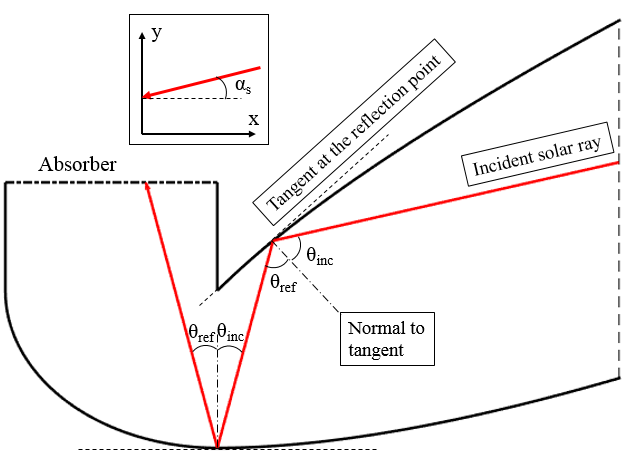
\includegraphics[width=\textwidth]{figs/RTvisual1}
%		\caption{Visualisation of one ray coming through the aperture at a certain angle $\alpha_s$ getting reflected at the upper parabolic and at the circular reflectors. $\theta_{inc}$ is the incident angle and $\theta_{ref}$ is the reflected angle.}
%		\label{RTvisual1}
%	\end{minipage} \hfill
%	\begin{minipage}[h]{0.475\linewidth}
%		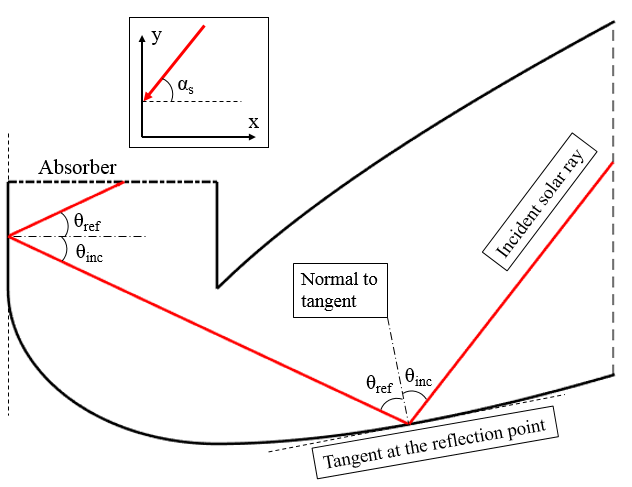
\includegraphics[width=\textwidth]{figs/RTvisual2}
%		\caption{Visualisation of one ray coming through the aperture at a certain angle $\alpha_s$ getting reflected at the lower parabolic and at the tertiary section reflectors.}
%		\label{RTvisual2}
%	\end{minipage}		
%\end{figure}

%\Figure[scale=0.5,placement=!ht,label={2D-diagram-1},caption={Visualisation in 2D of six rays coming through the aperture at an angle $\alpha_{\rm{s}}$.}]{figs/2D-diagram-1.eps}

%\Figure[scale=0.7,placement=!ht,label={3D-diagram-1},caption={Visualisation in 3D of two sets of six rays coming through the aperture at a particular pair of angles $\alpha_{\rm{s}}$ and $\gamma_{\rm{s}}$.}]{figs/3D-diagram-1.eps}

%For the modelling, it is important to check whether the incoming rays are reaching the absorber. This can be done by defining the angular acceptance, which is the ratio of the number of accepted rays to the total number of rays at a particular altitude solar angle ($\alpha_{\rm{s}}$), according to Eq. (\ref{ang_acc2}).

%\begin{equation}
%\mathrm{{\theta_{acc}} = \frac{{\mathlarger{\sum\limits}_{\scriptscriptstyle i = 1}^{{\scriptscriptstyle N_{rays}}} {{r_{acc}}(i)} }}{{{N_{rays}}}}}
%\label{ang_acc2}
%\end{equation}

%\noindent where the ray acceptance $\rm{r_{acc}(i)}$ for each ray i assumes only one of two possible values shown in Eq. (\ref{ang_acc1}):

%\begin{equation}
%\mathrm{{r_{acc}}(i)} = \left\{ \begin{array}{l}
%1{\rm{, \ if \ ray \ i \ reaches \ the \ absorber}}\\
%0{\rm{, \ if \ ray \ i \ does \ not \ reach \ the \ absorber}}
%\end{array} \right.
%\label{ang_acc1}
%\end{equation}

%The next step is to regard the reflective efficiency. This variable is defined as the ratio between the energy reaching the absorber and the incoming energy, considering only the reflection losses. It is calculated by Eq. (\ref{reflective}) and is a function of the concentrator's shape and the concentration ratio (\cite{Sellami2013}):

%\begin{equation}
%\mathrm{\eta_{\!_R} = \frac{\mathlarger{\sum\limits}_{\scriptscriptstyle i=1}^{\scriptscriptstyle N_{rays}}{{e_i}{\rho ^{{r_i}}}}}{{\mathlarger{\sum\limits}_{\scriptscriptstyle i=1}^{\scriptscriptstyle N_{rays}}{{e_i}}}}}
%\label{reflective}
%\end{equation}

%\noindent where $\rm{r_i}$ is the number of reflections of the solar ray i. It must be highlighted that each value of $\eta_{\rm{\!_R}}$ is calculated for each pair of $\alpha_{\rm{s}}$ and $\gamma_{\rm{s}}$. 
%Eq. \ref{globalreflective} shows how to estimate the average reflective efficiency, which is the average of all $\eta_{\rm{\!_R}}$ within the period of operation:

%\begin{equation}
%\mathrm{\eta_{\!_{R,avg}} = \frac{{\mathlarger{\int\limits}_{n_{\!_1}}^{n_{\!_2}} {\mathlarger{\int\limits}_{\omega_{\!_{s1}}}^{\omega_{\!_{s2}}} {{\eta_{\!_R}}d{\omega_s}dn} } }}{{\mathlarger{\int\limits}_{n_{\!_1}}^{n_{\!_2}} {\mathlarger{\int\limits}_{\omega_{\!_{s1}}}^{\omega_{\!_{s2}}} {d{\omega_s}dn}}}}}
%\label{globalreflective}
%\end{equation}

%\begin{equation}
%\mathrm{\tau_{g,avg} = \frac{{\mathlarger{\int\limits}_{n_{\!_1}}^{n_{\!_2}} {\mathlarger{\int\limits}_{\omega_{\!_{s1}}}^{\omega_{\!_{s2}}} {{\tau_{g}}d{\omega_s}dn} } }}{{\mathlarger{\int\limits}_{n_{\!_1}}^{n_{\!_2}} {\mathlarger{\int\limits}_{\omega_{\!_{s1}}}^{\omega_{\!_{s2}}} {d{\omega_s}dn}}}}}
%\label{globaltransmittance}
%\end{equation}

%\noindent where the transmittance $\tau_{\rm{g}}$ depends on the incident angle $\theta_{\rm{i}}$, which is the angle between the incident solar ray and the normal to the glazing, is calculated by Eq. (\ref{incidence}):

%Considering the operation period, Eq. (\ref{globaleta0}) expresses the calculation of the average optical efficiency:

%\begin{equation}
%\mathrm{{\eta_{o,avg}} = \frac{{\mathlarger{\int\limits}_{n_{\!_1}}^{n_{\!_2}} {\mathlarger{\int\limits}_{\omega_{\!_{s1}}}^{\omega_{\!_{s2}}} {{\eta_{o}}d{\omega_s}dn} } }}{{\mathlarger{\int\limits}_{n_{\!_1}}^{n_{\!_2}} {\mathlarger{\int\limits}_{\omega_{\!_{s1}}}^{\omega_{\!_{s2}}} {d{\omega_s}dn}}}}}
%\label{globaleta0}
%\end{equation}

%The algorithm in 2D followed the steps depicted in Figure (\ref{RT3D}).
%
%\Figure[scale=0.80,placement=!ht,label={RT3D},caption={Simulation procedure flowchart of the 2D ray tracing algorithm.}]{figs/RT3D.png}

%Considering the operation period, Eq. (\ref{globalCeff}) expresses the calculation of the average effective concentration ratio:

%\begin{equation}
%\mathrm{{C_{eff,avg}} = \frac{{\mathlarger{\int\limits}_{n_{\!_1}}^{n_{\!_2}} {\mathlarger{\int\limits}_{\omega_{\!_{s1}}}^{\omega_{\!_{s2}}} {{C_{eff}}d{\omega_s}dn} } }}{{\mathlarger{\int\limits}_{n_{\!_1}}^{n_{\!_2}} {\mathlarger{\int\limits}_{\omega_{\!_{s1}}}^{\omega_{\!_{s2}}} {d{\omega_s}dn}}}}}
%\label{globalCeff}
%\end{equation}

%From those values of parabola axis angles, the maximum concentration ratio achieved was 2.28.

%Using SolidWorks, the sketch of the initial design was performed (shown in Figure \ref{col1}) and from this, the absorber width was found with the aim of achieving the maximum concentration ratio. Hence, the absorber width ($\rm{W_{abs}}$) is 145 mm with the concentration ratio is 2.28.


%\subsection{Design analysis and optical performance of standalone collector}

%whereas the dimensionless of width and height varied from 3.2 to 7 times the absorber width. Geometries of smaller values of $\alpha_{\!_{\rm{P2}}}$ are optically less efficient because they do not accept part of direct radiation at high solar altitude angles. At $\alpha_{\!_{\rm{P2}}} > 59^{\circ}$ There is little increase in the optical efficiency because the shapes already accept all the direct radiation of the operation period. For the effective concentration ratio, there is a geometry that maximises this variable.

%is less than 0.45 for the geometry of $\alpha_{\!_{\rm{P1}}}$ = 45$^{\circ}$ because it does not accept any direct radiation of $\alpha_{\rm{s}}$ > 45$^{\circ}$.

%This region of $\alpha_{\!_{\rm{P2}}}$ and $\alpha_{\!_{\rm{P1}}}$ = 17$^{\circ}$ ensures that

%\Figure[scale=0.5,placement=!ht,label={size_full},caption={Dimensionless parameter as function of the lower parabola axis angle.}]{figs/size_full.png}

%From the optical analysis of these shapes of maximum CR, the average optical efficiency also increases as $\alpha_{\!_{\rm{P2}}}$ increases because more direct solar radiation is accepted at high solar altitude angles until the condition where all the radiation from the period of operation is collected. It was observed that the shape where $\alpha_{\!_{\rm{P2}}} = 56^{\circ}$ results in the maximum effective concentration ratio ($\rm{C_{eff} = 1.57}$) even though only a portion of direct radiation of altitude angle above $56^{\circ}$ is accepted. At this condition, CR = 2.42, average $\rm{\eta_o = 0.647, W^* = 4.57}$ and $\rm{H^* = 3.84}$. Considering a concentrator of 100 mm in $\rm{W_{abs}}$, the total reflector area required is 1.36 $\rm{m^2}$.

%\Figure[scale=0.5,placement=!ht,label={efficiency_full},caption={Optical efficiency and effective concentration ratio vs lower parabola axis angle.}]{figs/efficiency_full.png}

%\subsection{Effect of the parabolic shape and tertiary section}

%In the operation period, the limits of altitude solar angle calculated by Eq. (\ref{solar_alt}) are:

%\begin{itemize}
%	\item 60$^{\circ}$ as the upper limit, when the Sun is at its highest altitude, in the summer solstice (21/06) at solar noon;
%	\item 17$^{\circ}$ as the lower limit, when the Sun is at its lowest altitude in the equinox (21/09) at 8 am (9 am in summertime).
%\end{itemize}

%The concentrator's aperture is set at the vertical position (at the truncation line indicated in Figure \ref{CSview}) so that shading can be avoided when two or more collectors are stacked on a wall. The actual aperture width ($\rm{W_{apt}}$) will be 330 mm in order to have three collectors stacked on every metre of wall height. The glazing placed in the primary section works as a heat trap, as well as offering protection for the interior of the unit against weather conditions. Its position at a given inclination $\beta$ seeks to maximise light transmittance over the operation period considered.

%\Figure[scale=0.65,placement=!ht,label={col1},caption={Concentrator's initial design.}]{figs/col1.eps}



%\subsection{Evaluation of the length on the optical performance}

%For the length analysis, the average reflective efficiency () was calculated at different collector lengths and therefore Figure \ref{length1} shows the relationship between these two variables.

%\Figure[scale=0.65,placement=!ht,label={length1},caption={Average reflective efficiency \textit{vs.} $\rm{L_{col}}$.}]{figs/length.eps}

%There is an increase in efficiency up to \mbox{$\rm{L_{col}}$ = 0.625 m} with only a slight increase above that, thus longer collectors are more efficient. This is due to a smaller number of reflections incident on the end plates, enhancing optical performance. This analysis is important to decide how long a collector must be considering the amount of material for its fabrication. From the design, the reflector weight and cost were calculated as function of $\rm{L_{col}}$ and shown in Figure \ref{cost-weight}. It is important to remark that the end plates are included, and the cost was calculated based on 50 euro per m$^2$ of reflector sheet.

%\Figure[scale=0.65,placement=!ht,label={cost-weight},caption={Cost and weight of reflector as function of the collector length.}]{figs/cost-weight.eps}

%The reflective efficiency at $\rm{L_{col}}$ = 0.625 m is 0.890 whereas the same efficiency at 1.25 m in length is 0.905. It is a gain in efficiency of 1.5\%, but at the cost of 76\% more material for the collector fabrication. The manufacturer may opt to fabricate two 0.625-m long collectors instead of one with 1.25 m in length.

%To understand the effect of the cavity height in the optical analysis, the average reflective efficiency calculated by Eq. (\ref{reflective}) is shown in Figure \ref{TSanalysis} as function of the tertiary section height. For this analysis, $\alpha_{\!_{\rm{P2}}}$ was kept at 50$^{\circ}$.

%\Figure[scale=0.55,placement=!ht,label={TSanalysis},caption={Average reflective efficiency {\itshape versus} tertiary section height for 2D and 3D models.}]{figs/TSanalysis.eps}

%Both graphs of $\rm{\overline \eta_{\!_R}}$ have an approximate linear behaviour. The drop in efficiency as $\rm{H_{\!_{TS}}}$ increases is due to the higher number of reflections. The difference between both graphs is approximately 2\%, where the 3D model resulted in smaller values of $\rm{\overline \eta_{\!_R}}$ as the reflections at the ends are taken into account.

%Although the optical efficiency is reduced by the increase of the tertiary section height, the cavity has a function of distributing the incoming energy uniformly along the absorber surface. To apply this function, the results of the simulation $\alpha_{\rm{s}}$ at 54$^{\circ}$ was selected and this can be seen in Figs. \ref{TS0-2}, \ref{TS72-2} and \ref{TS145-2}.

%\begin{figure}[ht!]
%	\begin{minipage}{0.40\columnwidth}
%		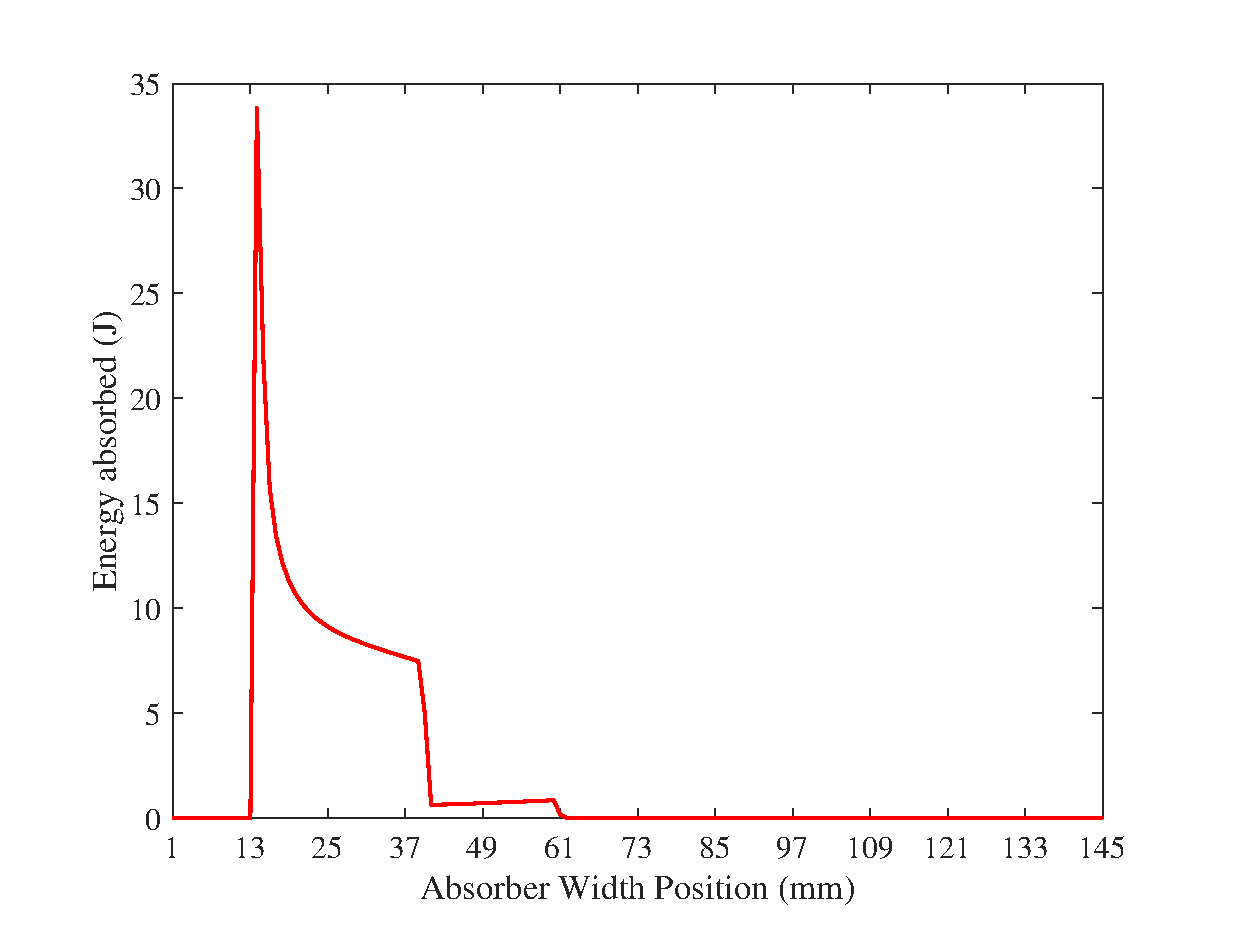
\includegraphics[width=0.95\columnwidth,height=4.2cm]{figs/TS0_Energy.eps}
%		\subcaption{Energy distribution.}
%		
%		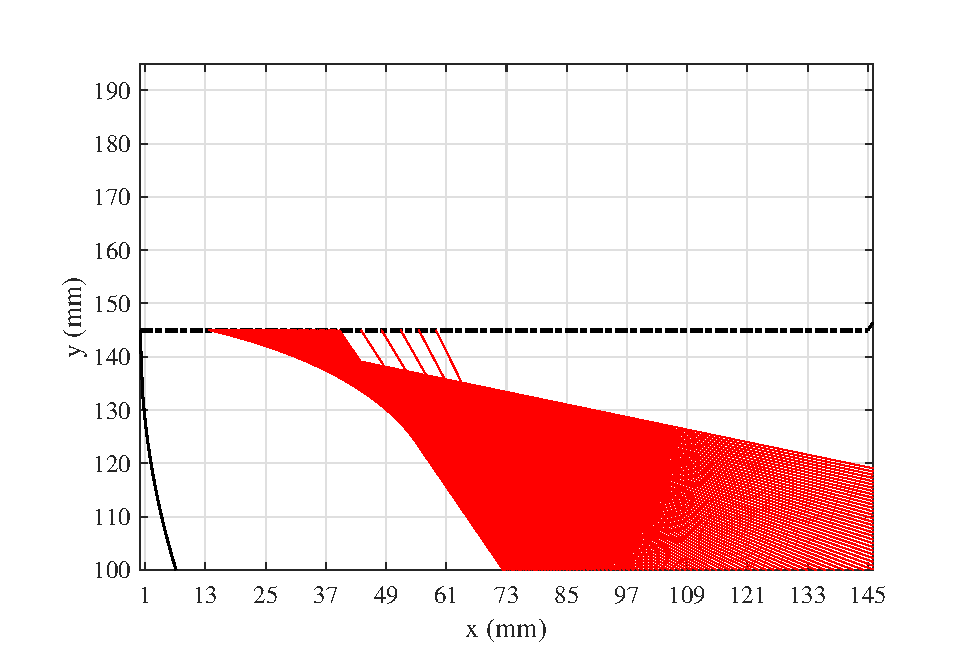
\includegraphics[width=0.95\columnwidth,height=4.1cm]{figs/TS0-22.eps}
%		\subcaption{Absorber width magnified.}
%	\end{minipage}
%	\begin{minipage}{0.59\columnwidth}
%		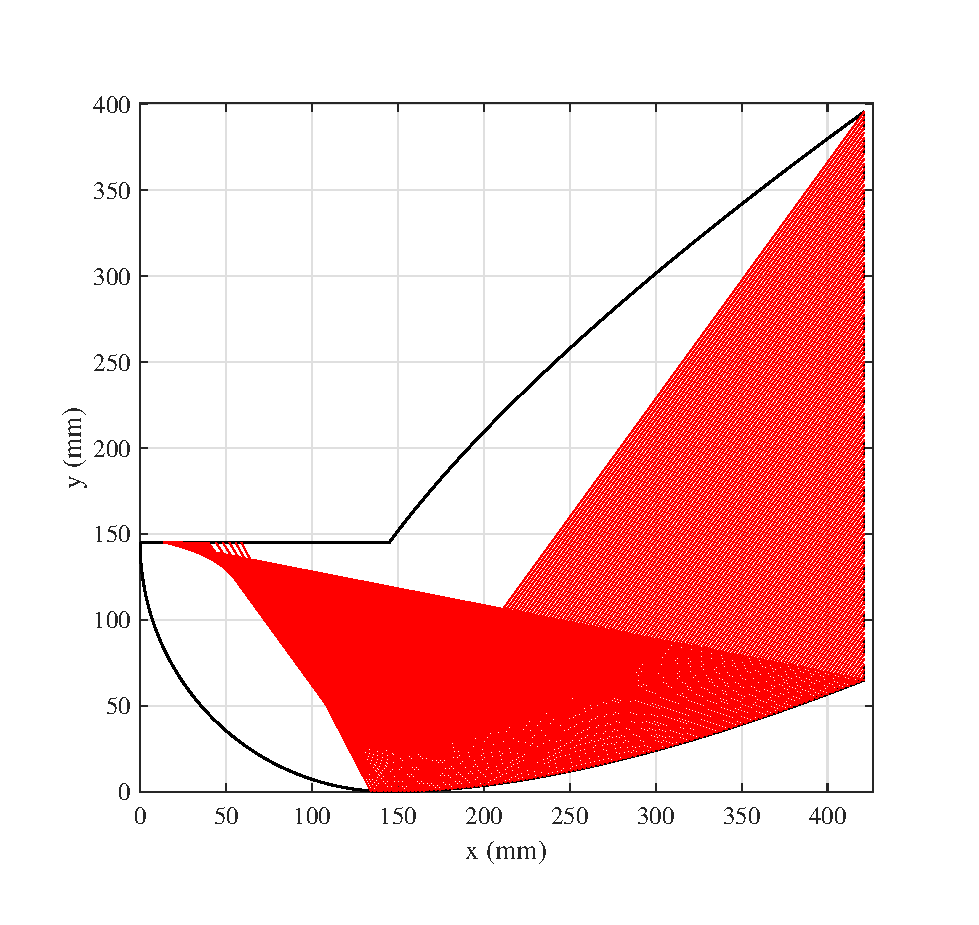
\includegraphics[width=0.95\columnwidth,height=85mm]{figs/TS0-1.eps}
%		%\\[-9mm]
%		\subcaption{Ray tracing diagram.}
%	\end{minipage}
%	\caption{Ray tracing diagram in 2D and energy distribution over the absorber width with no tertiary section.}
%	\label{TS0-2}
%\end{figure}
%
%%\Figure[scale=0.70,placement=!ht,label={TS0-2},caption={Ray tracing diagram in 2D and energy distribution over the absorber width with no tertiary section.}]{figs/TS0-2.png}
%
%\begin{figure}[ht!]
%	\begin{minipage}{0.40\columnwidth}
%		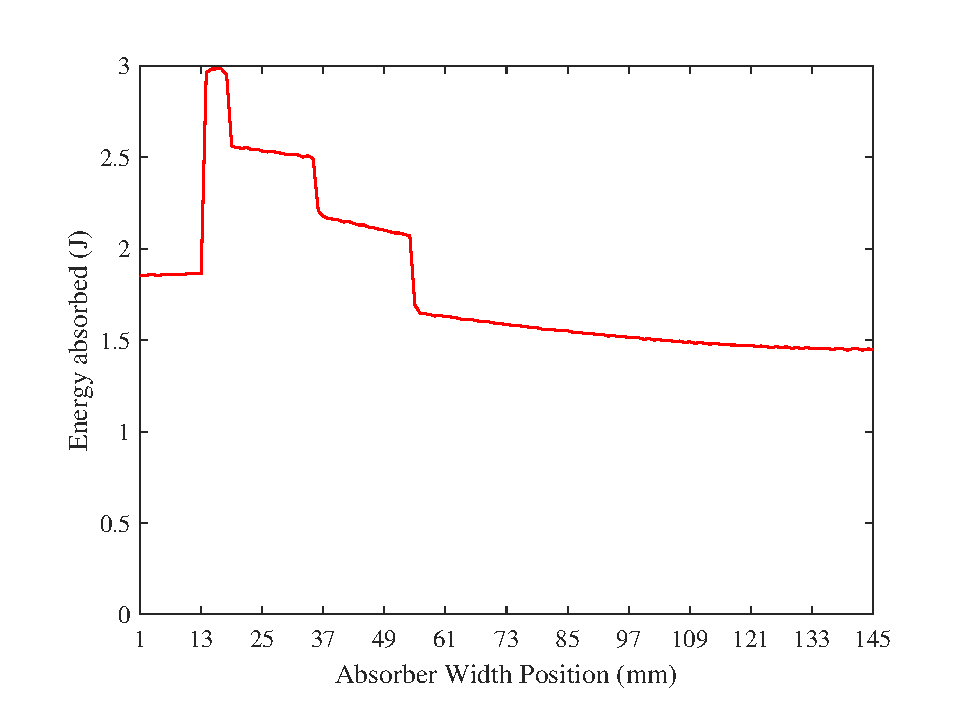
\includegraphics[width=0.95\columnwidth,height=4.2cm]{figs/TS72-Energy.eps}
%		\subcaption{Energy distribution.}
%		
%		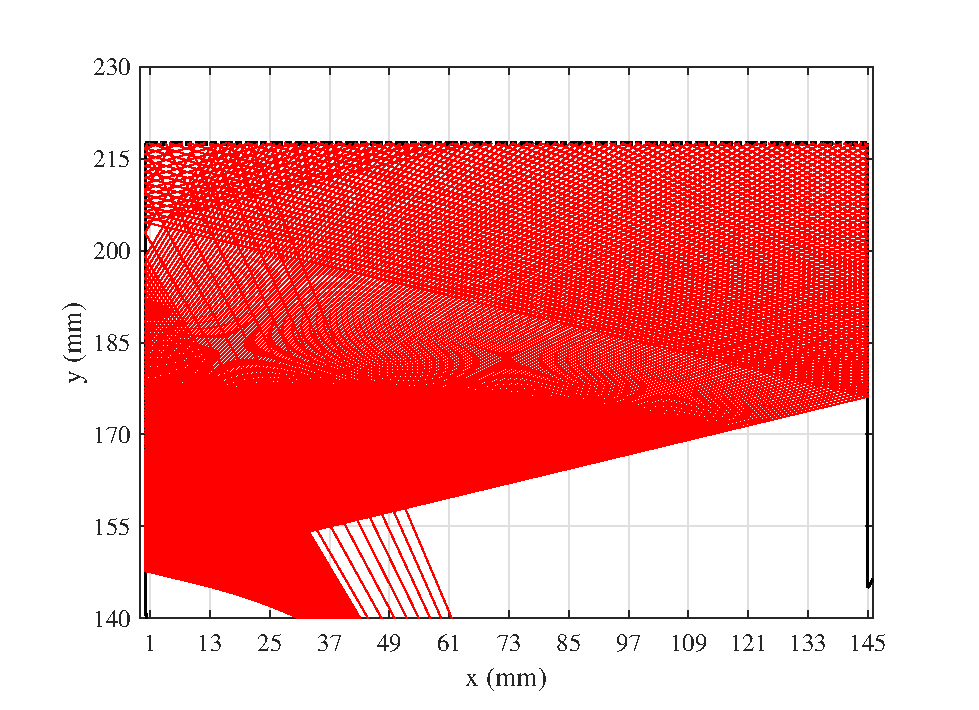
\includegraphics[width=0.95\columnwidth,height=4.1cm]{figs/TS72-22.eps}
%		\subcaption{Absorber width magnified.}
%	\end{minipage}
%	\begin{minipage}{0.59\columnwidth}
%		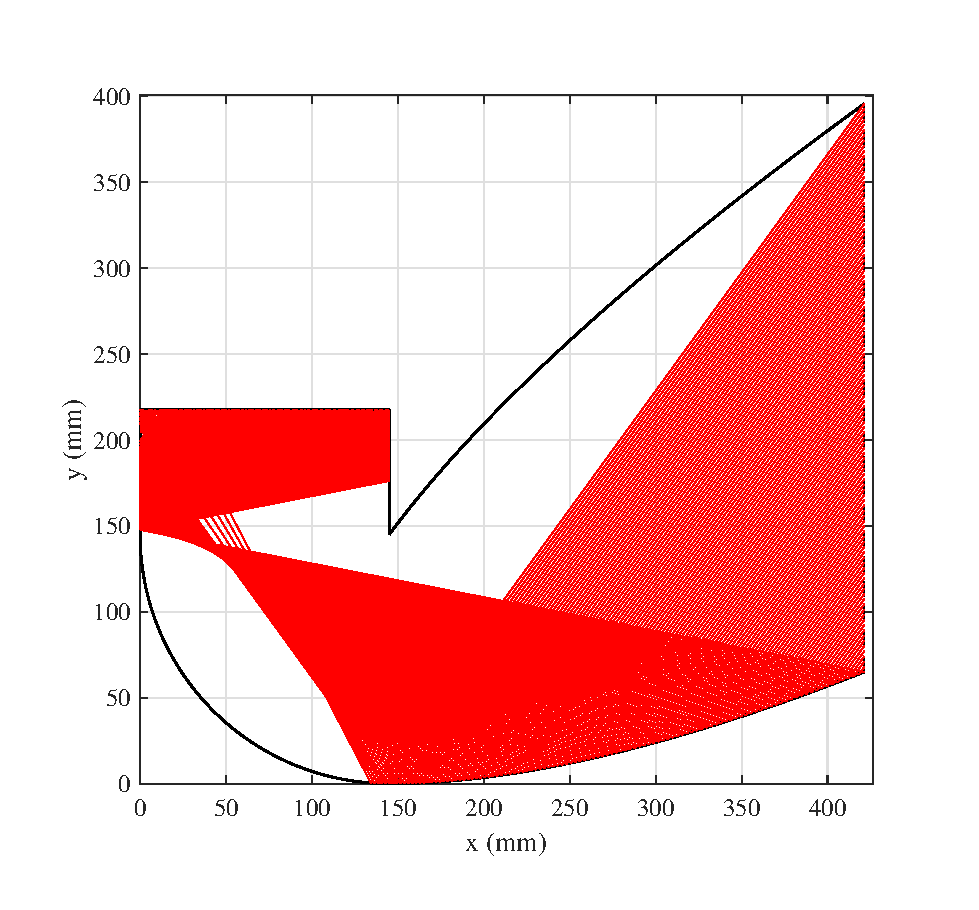
\includegraphics[width=0.95\columnwidth,height=85mm]{figs/TS72-1.eps}
%		%\\[-9mm]
%		\subcaption{Ray tracing diagram.}
%	\end{minipage}
%	\caption{Ray tracing diagram in 2D and energy distribution over the absorber width at 72.5 mm of tertiary section.}
%	\label{TS72-2}
%\end{figure}
%
%%\Figure[scale=0.70,placement=!ht,label={TS72-2},caption={Ray tracing diagram in 2D and energy distribution over the absorber width at 72.5 mm of tertiary section.}]{figs/TS72-2.png}
%
%\begin{figure}[ht!]
%	\begin{minipage}{0.40\columnwidth}
%		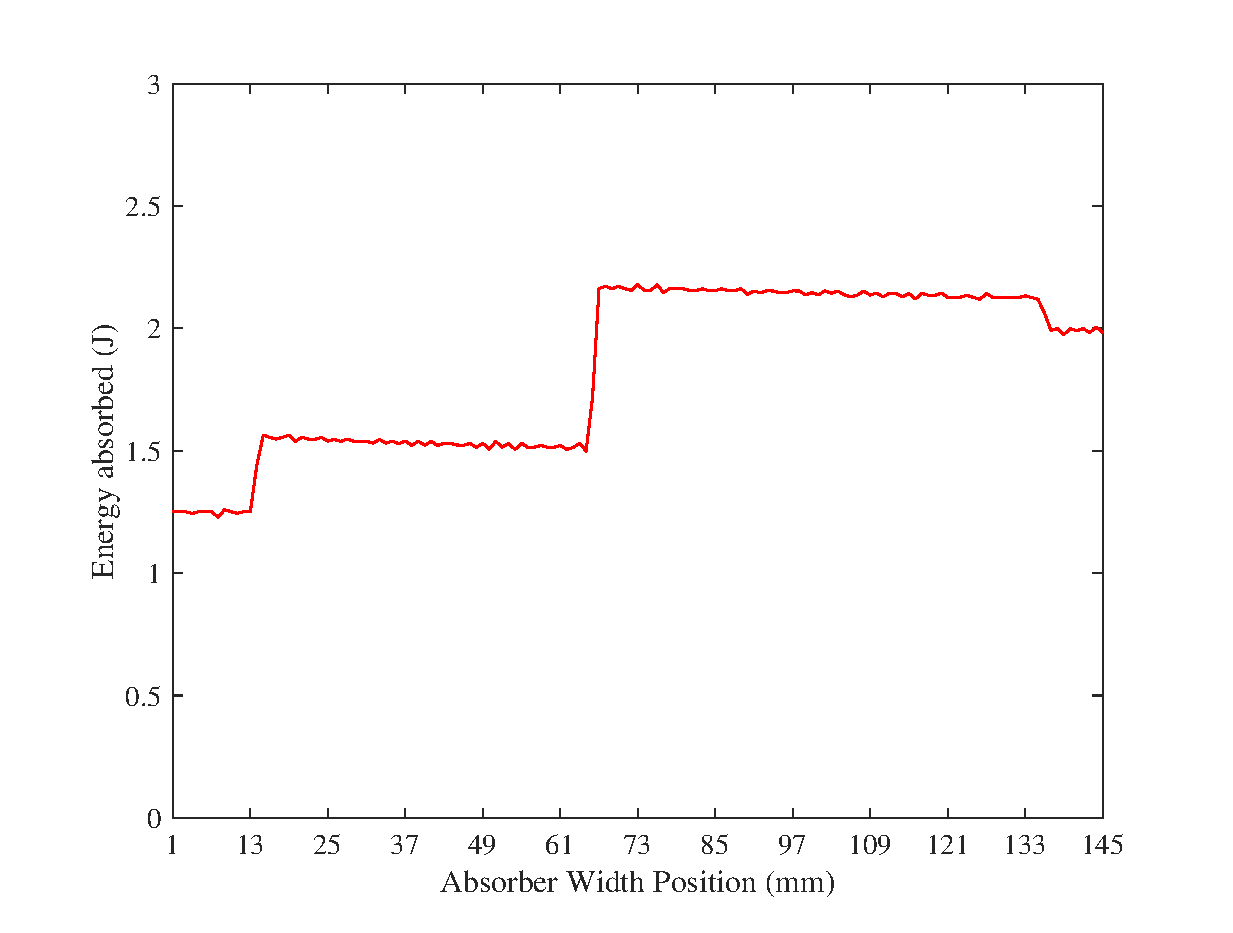
\includegraphics[width=0.95\columnwidth,height=4.2cm]{figs/TS145-Energy.eps}
%		\subcaption{Energy distribution.}
%		
%		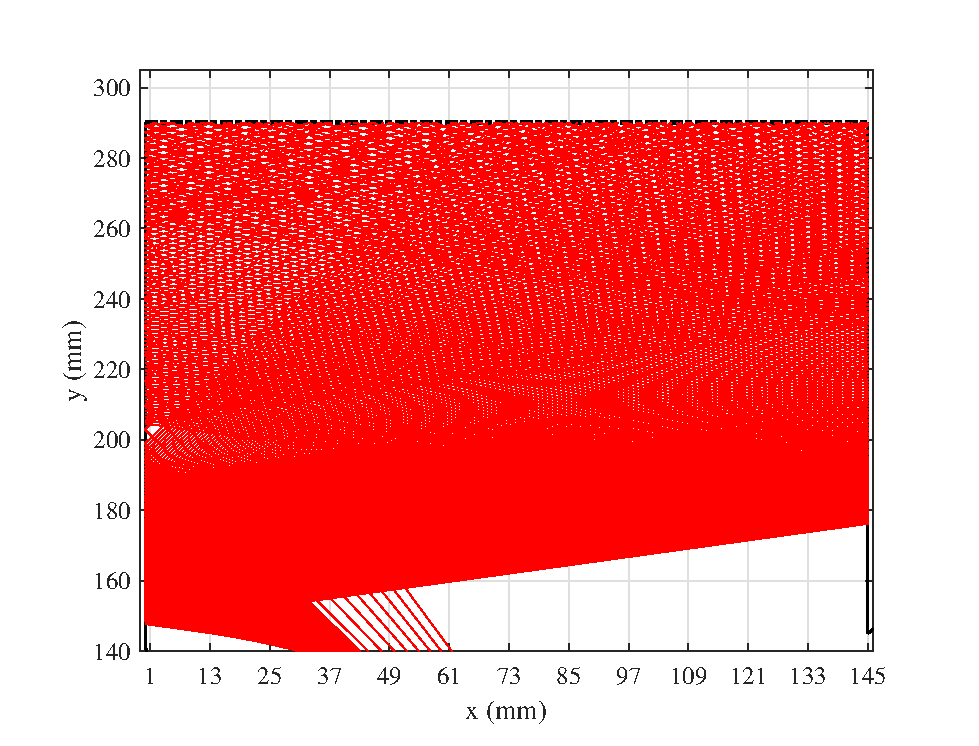
\includegraphics[width=0.95\columnwidth,height=4.5cm]{figs/TS145-22.eps}
%		\subcaption{Absorber width magnified.}
%	\end{minipage}
%	\begin{minipage}{0.59\columnwidth}
%		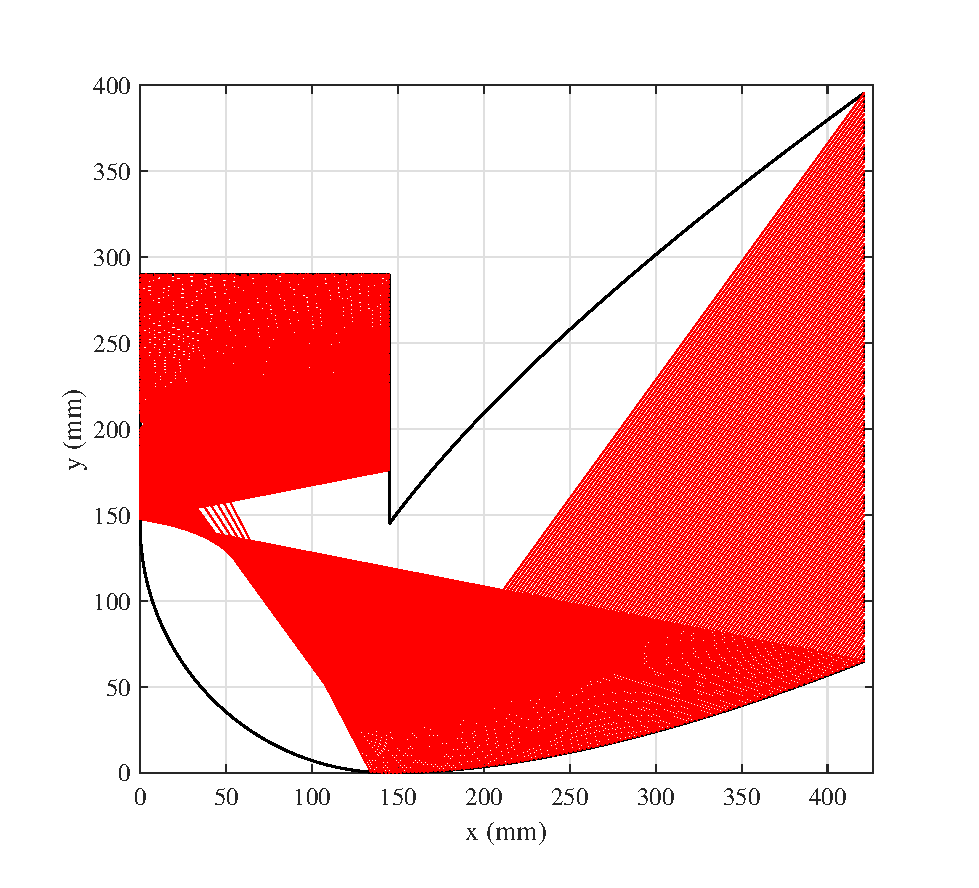
\includegraphics[width=0.95\columnwidth,height=85mm]{figs/TS145-1.eps}
%		%\\[-9mm]
%		\subcaption{Ray tracing diagram.}
%	\end{minipage}
%	\caption{Ray tracing diagram in 2D and energy distribution over the absorber width at 145 mm of tertiary section.}
%	\label{TS145-2}
%\end{figure}
%
%%\Figure[scale=0.70,placement=!ht,label={TS145-2},caption={Ray tracing diagram in 2D and energy distribution over the absorber width at 145 mm of tertiary section.}]{figs/TS145-2.png}

%From Figure \ref{TS0-2}, a high energy peak concentrated in one millimetre of absorber width is observed and all the energy is concentrated in 45 millimetres. From Figs. \ref{TS72-2} and \ref{TS145-2}, the energy is more distributed across the absorber surface. Hence, the tertiary section helps to distribute the solar energy more uniformly over the absorber area, which is desirable for further heat transfer even though the reflection losses are higher.
